\documentclass[11pt]{beamer}
\usepackage[utf8]{inputenc}
\usepackage[T1]{fontenc}
\usepackage{amsmath}
\usepackage{amsfonts}
\usepackage{amssymb}
\usepackage{graphicx}
\usetheme{default}
\usepackage{subfig}

\begin{document}
	\author{Musa Baloyi}
	\title{Model governance for risk management}
	%\subtitle{The what and why of logging, monitoring and documentation}
	%\logo{}
	\titlegraphic{
\includegraphics[width=\textwidth,height=.5\textheight]{images/sbsa_logo}}
	%\institute{}
	%\date{\today}
	%\subject{}
	%\setbeamercovered{transparent}
	%\setbeamertemplate{navigation symbols}{}
	\begin{frame}[plain]
	\maketitle
\end{frame}


\begin{frame}
\frametitle{Table of contents}
\begin{itemize}
	\item Model definition, uses, examples, decisions, lifecycle
	\item Regulatory expectations: of models, of institution senior management
	\item Model risk, ranking, components, sources, teams%, model risk governance framework
	\item Model governance: uses, life cycle, best practices, key roles, key elements, framework
	\item To come: model inventory, model monitoring, model validation
	%\item Model inventory, enterprise level model inventory, complexity
	%\item Monitoring, key principles of effective model monitoring
	%\item Model validation
%	\item Effective management information systems (MIS), Credit risk model monitoring suite
\end{itemize}
\end{frame}

\begin{frame}
\begin{figure}[h]
	\centering
	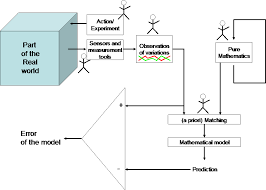
\includegraphics[scale=.7]{images/model}
\end{figure}
\centering
Model definition, uses, examples, decisions, lifecycle
\end{frame}

\begin{frame}
\frametitle{What is a model?}
\begin{itemize}
%	\item Stadard Bank Group consensus of model.
	\item A quantitative method, system, or approach that applies statistical, economic, financial, or mathematical theories, techniques, and assumptions to process input data into quantitative estimates or output. (SR 11-7)
	\item Also covers quantitative approaches whose inputs are partially or wholly qualitative or based on expert judgment, provided that the output is quantitative in nature. (SR 11-7)
	% In addition, models play a direct role in determining regulatory capital requirements at many of the nation’s largest and most complex banking organizations. Some of these institutions already use value-at-risk models to determine regulatory capital held for market risk exposure. 
	% At institutions adopting the Basel II capital standards when finalized, financial models will have a much expanded role in establishing regulatory capital held for all risk types.
	\item Not all models involve complex mathematical techniques or require detailed computer programming code.
	% This does not, however, diminish their potential importance to the organization.
	% Although at first glance this may not appear to be a “model,” the output from such spreadsheets directly contributes to preparation of the institution’s reported financial statements, and some controls are necessary, given the seriousness of any potential errors.	
	\item Financial models describe business activity, predicting future or otherwise unknown aspects of that activity. 
\end{itemize}
\end{frame}


\begin{frame}
\frametitle{Uses of models in the banking industry}
\begin{itemize}
	\item setting the business strategy, 
	\item informing decision making, 
	\item measuring risk, 
	\item managing risk, 
	\item monitoring and setting internal limits, 
	\item calculating exposures, 
	\item pricing different instruments, 
	\item performing stress testing, 
	\item calculating regulatory capital, 
	\item estimating asset values, etc.
\end{itemize}
% Asset Liability Management (ALM), valuation, risk measurement, asset allocation and hedging.
% product pricing and risk segmentation; business planning; assumption development; cash flow testing analysis; financial reporting; appraisals of insurance businesses; asset adequacy analysis; life insurance illustrations; risk evaluations; and reserve calculations.
\end{frame}


\begin{frame}
\frametitle{Examples of models in the banking industry}
\begin{itemize}
	\item Credit scoring models %inform decision making, providing predictive information on the potential for default or delinquency used in the loan approval process and risk pricing
	\item Interest rate risk models %measure risk, monitoring earnings exposure to a range of potential changes in rates and market conditions
	\item Derivatives pricing models %estimate asset value, providing a methodology for determining the value of new or complex products for which market observations are not readily available
\end{itemize}
\end{frame}


\begin{frame}
\frametitle{Decisions that can be influenced through the use of models}
\begin{itemize}
	\item Setting the appropriate level of reserves a company should hold to fulfill its obligations;
	\item Setting the rates to charge for new business;
	\item Targeting specific products to sell;
	\item Exiting the market for certain products;
	\item Management of the in-force business, including the current premiums, cost of insurance (COIs), credited rates, dividend scales, and replacement programs;
	\item Incorporating risk mitigation such as reinsurance agreements;
	\item Management of capital resources.
\end{itemize}
\end{frame}


\begin{frame}
\frametitle{Model life cycle}
Model risk may pop up at any stage during the life cycle of a specific model.
\begin{figure}[h]
	\centering
	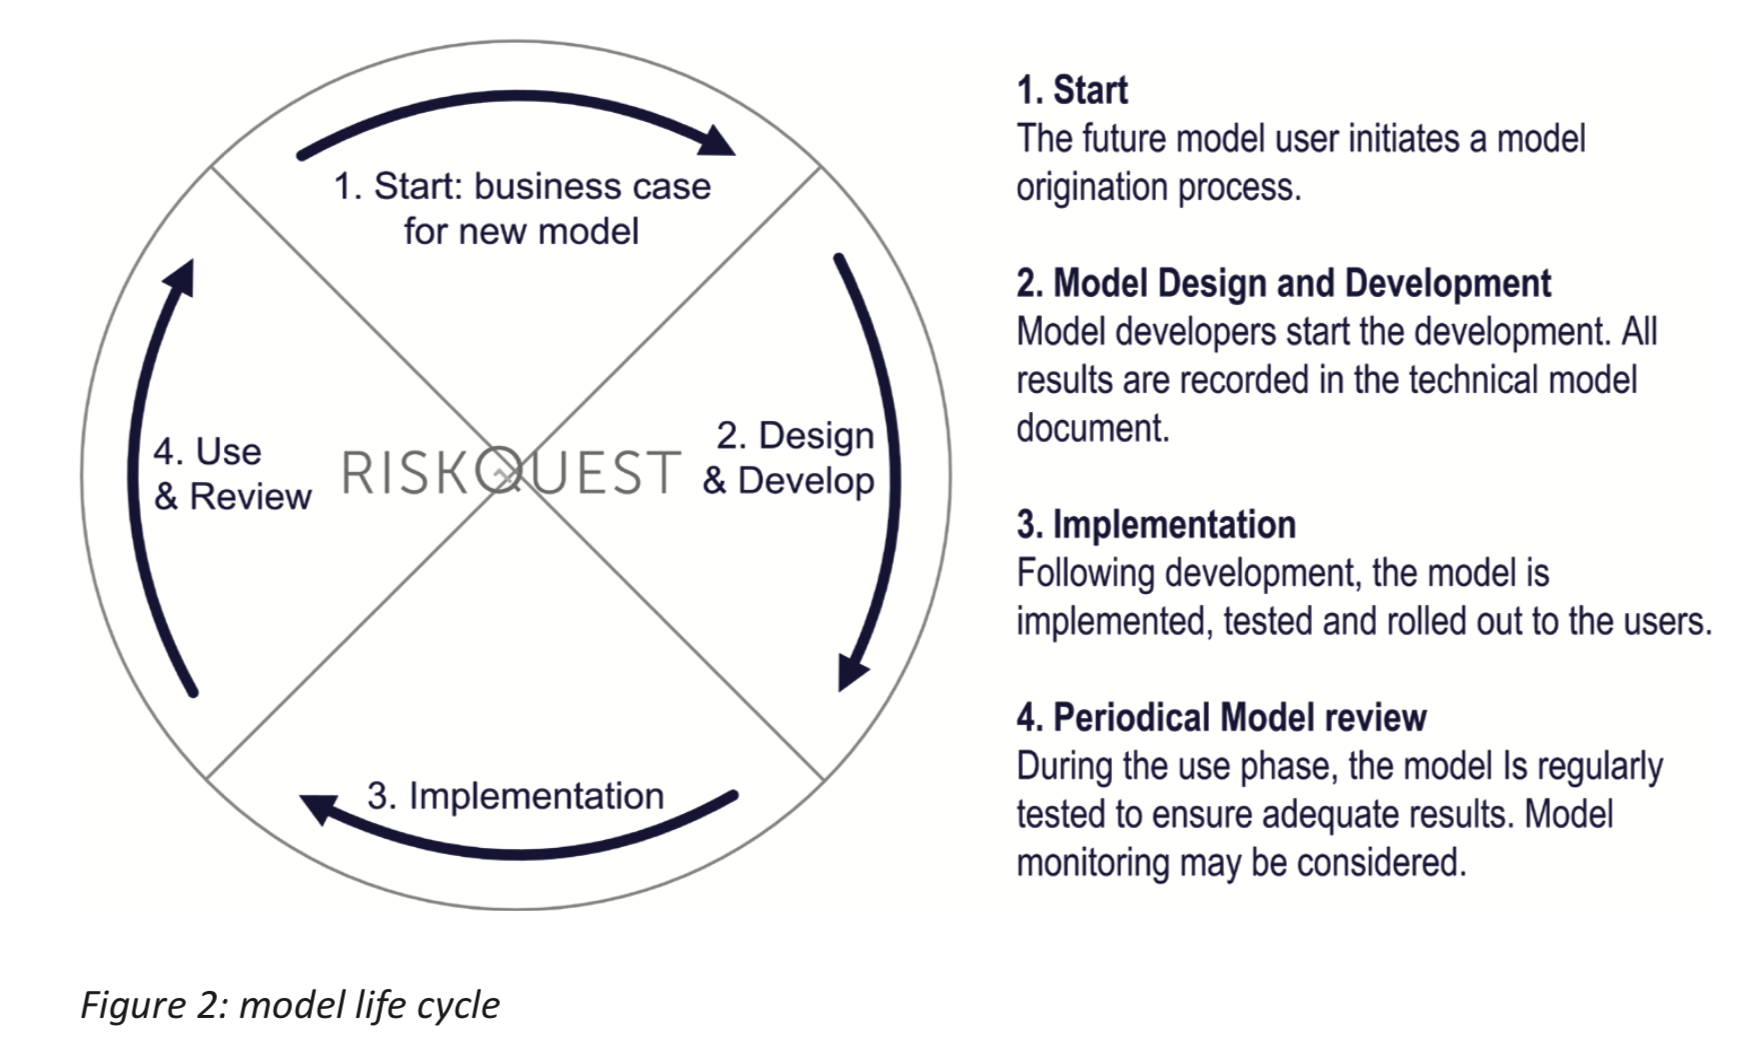
\includegraphics[scale=.3]{images/model_lifecycle}
\end{figure}
\end{frame}


\begin{frame}
\frametitle{Model development life cycle}
\begin{itemize}
	\item Define and develop specifications for the model;
	\item Develop or modify code/program the model;
	\item Test/validate the model;
	\item Approve the model for implementation; and
	\item Validate that controls are in place and documentation is complete.
\end{itemize}
\end{frame}


\begin{frame}
\centering
Regulatory expectations: of models, of institution senior management
\end{frame}

\begin{frame}
\frametitle{Regulatory expectations of models}
\begin{itemize}
	\item Since the last financial crisis, there has been ever increasing regulatory pressure over the appropriateness of models. 
	\item Regulations question the appropriateness of models wrt:
	\begin{itemize}
		\item assumptions and limitations of models, 
		\item quality of data used for calibration, 
		\item thoroughness and independence of the validation process,
		\item robustness of policies, processes and controls, 
		\item use tests, 
		\item quality of model documentation.
	\end{itemize}
	%\item In addition to responding to regulatory pressure, 
	\item Banks should closely look at their models to protect their business and its reputation.
\end{itemize}
\end{frame}


\begin{frame}
\frametitle{Regulatory expectations of institution senior management}
\begin{itemize}
%An institution’s senior management should be in a position to 
	\item Understand the limitations of models, regardless of where the limitations come from, e.g.
	\begin{itemize}
		\item Methodological underpinnings
		\item Quality and availability of data used for calibration
		\item Limitations linked to the models’ implementation (numerical inaccuracies, technological issues, source code bugs, etc.)
		\item Limitations imposed by the context in which the model will be used
	\end{itemize}
%Regulators also expect Senior management and model users to 
	\item Challenge the assumptions made by model developers.
	\item Question whether or not the models would be adequate in real-life situations.
%. In particular, 
	\item It should be clear under what circumstances the assumptions would no longer hold.
\end{itemize}
\end{frame}


\begin{frame}
\begin{figure}[h]
	\centering
	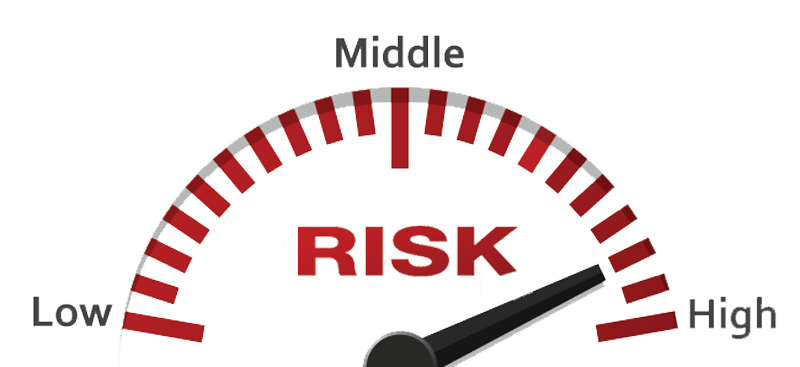
\includegraphics[scale=.4]{images/risk}
\end{figure}
\centering
Model risk, components, sources, ranking, teams
\end{frame}


\begin{frame}
\frametitle{Model risk}
\begin{itemize}
	\item Although the use of models as a management tool is a significant advance for the industry, the models themselves represent a new source of risk - the potential for model output to incorrectly inform management decisions.
	\item The application of models for decision making also exposes the institutions to a new form of risk, i.e. model risk. 
	\item This is the risk of financial loss or reputational damage resulting from weaknesses in the use of models. 
	\item Unlike other types of risk, model risk is a secondary type of risk in the sense that it is not rewarded.
	% Model risk can be introduced by any type of model within an organization, ranging from spreadsheet based models to complex IT solutions, from models used by the front office to models used by finance, from pricing models to ALM models.
	% To have effective model risk mitigation, also supporting systems and processes should be in scope, i.e. the functional operation of the end-to-end system against defined design docu- mentation and the traceability of data flows from source system to final output.
	% [t]he risk of adverse consequences resulting from reliance on a model that does not adequately represent that which is being modeled or that is misused or misinterpreted.
\end{itemize}
\end{frame}


\begin{frame}
\frametitle{Key risk components}
\begin{itemize}
	\item Financial impact;
	\item Regulatory, reputational, and operational impacts;
	\item Complexity of data and assumptions utilized;
	\item Complexity of the calculation engine;
	\item Complexity of the overall process, intuitiveness/transparency;
	\item Level of expertise/experience of the model developer and user.
\end{itemize}
\end{frame}


\begin{frame}
\frametitle{Sources of model risk}
\begin{figure}[h]
\centering
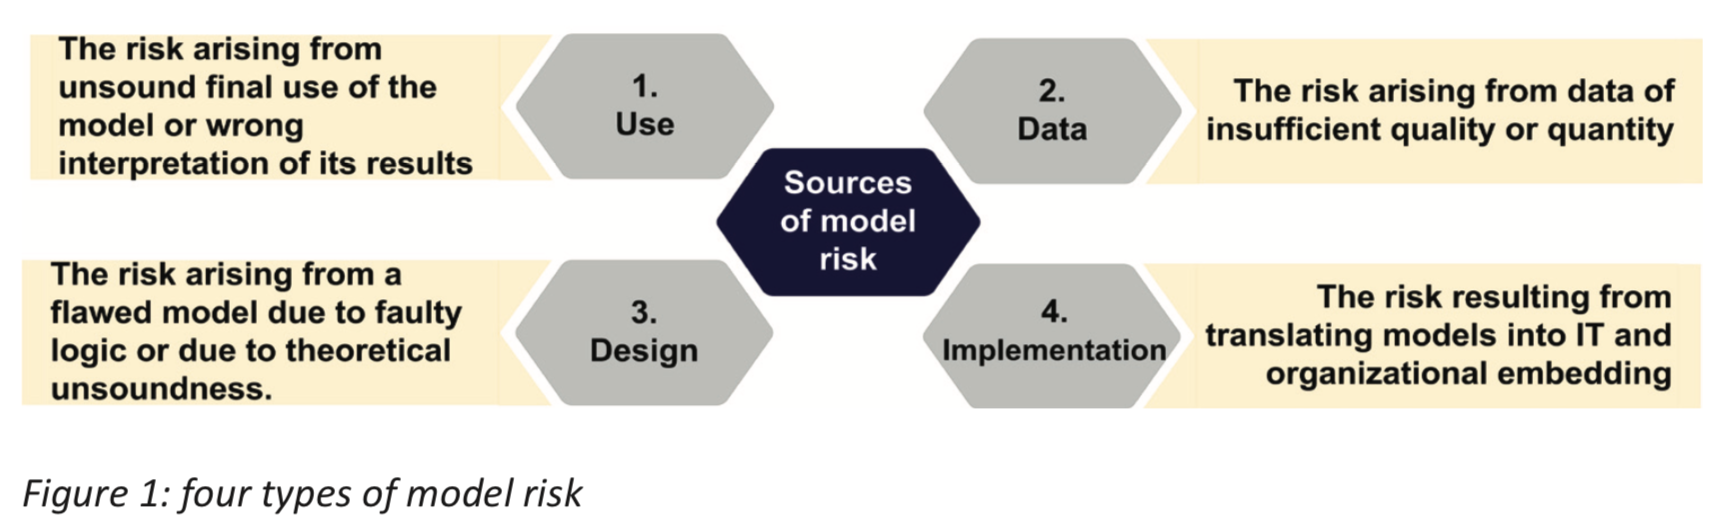
\includegraphics[scale=.35]{images/sources_of_model_risk}
\end{figure}
\end{frame}


\begin{frame}
\frametitle{Model risk ranking}
\begin{itemize}
\item The appropriateness of model use - “fit for purpose”;
\item The frequency and depth of model reviews;
\item The level of approval for new model development or when an old model is (substantially) revised;
\item The composition of a model review team.
\end{itemize}
\end{frame}


\begin{frame}
\frametitle{Model risk teams}
\begin{itemize}
\item Ideally, model risk teams, together with model validation teams, are independent of model development teams to avoid a conflict of interest.
\item Their mandate should cover all aspects of the development, calibration, validation, and implementation of the models, as well as the quality of the model results and reporting.
\item Challenge the effectiveness of the policies that affect the use of these models, review the robustness of the process used in data management, model calibration, and implementation, as well as the thoroughness of the controls.
\item Determine the required level of automation, which minimizes human error while allowing for reasonable judgment overrides.
\end{itemize}
\end{frame}


\begin{frame}
\frametitle{Model risk teams}
\begin{itemize}
\item Model risk teams should establish a process for approvals, including key stakeholders and sign ­off levels required before the model can be used (i.e., whether department/regional committee approval is enough or whether business line or even group level approvals are required).
\item Once the firm has accepted that the use of models carries a specific type of risk, this risk should be included in the firm’s risk appetite statement. In particular, budget approvals for modeling teams and critical investments on model, data, and reporting technology should be part of these discussions.
\end{itemize}
\end{frame}


\begin{frame}
\begin{figure}[h]
	\centering
	
\includegraphics[scale=.3]{images/governance}
\end{figure}
\centering
Model governance: uses, lifecycle, framework, key roles, key elements, best practices
\end{frame}


\begin{frame}
\frametitle{Model governance uses}
Although modeling necessarily involves the opportunity for error, strong governance procedures can help minimize model risk by
\begin{itemize}
	\item Providing reasonable assurance the model is operating as intended;
	\item Contributing to ongoing model improvement to maintain effectiveness;
	\item Promoting better management understanding of the limitations and potential weaknesses of a model.
\end{itemize}
Key purpose of model governance is to manage the set of models in such way as to reduce model risk.
\end{frame}


\begin{frame}
\frametitle{Model governance lifecycle}
\begin{figure}[h]
\centering
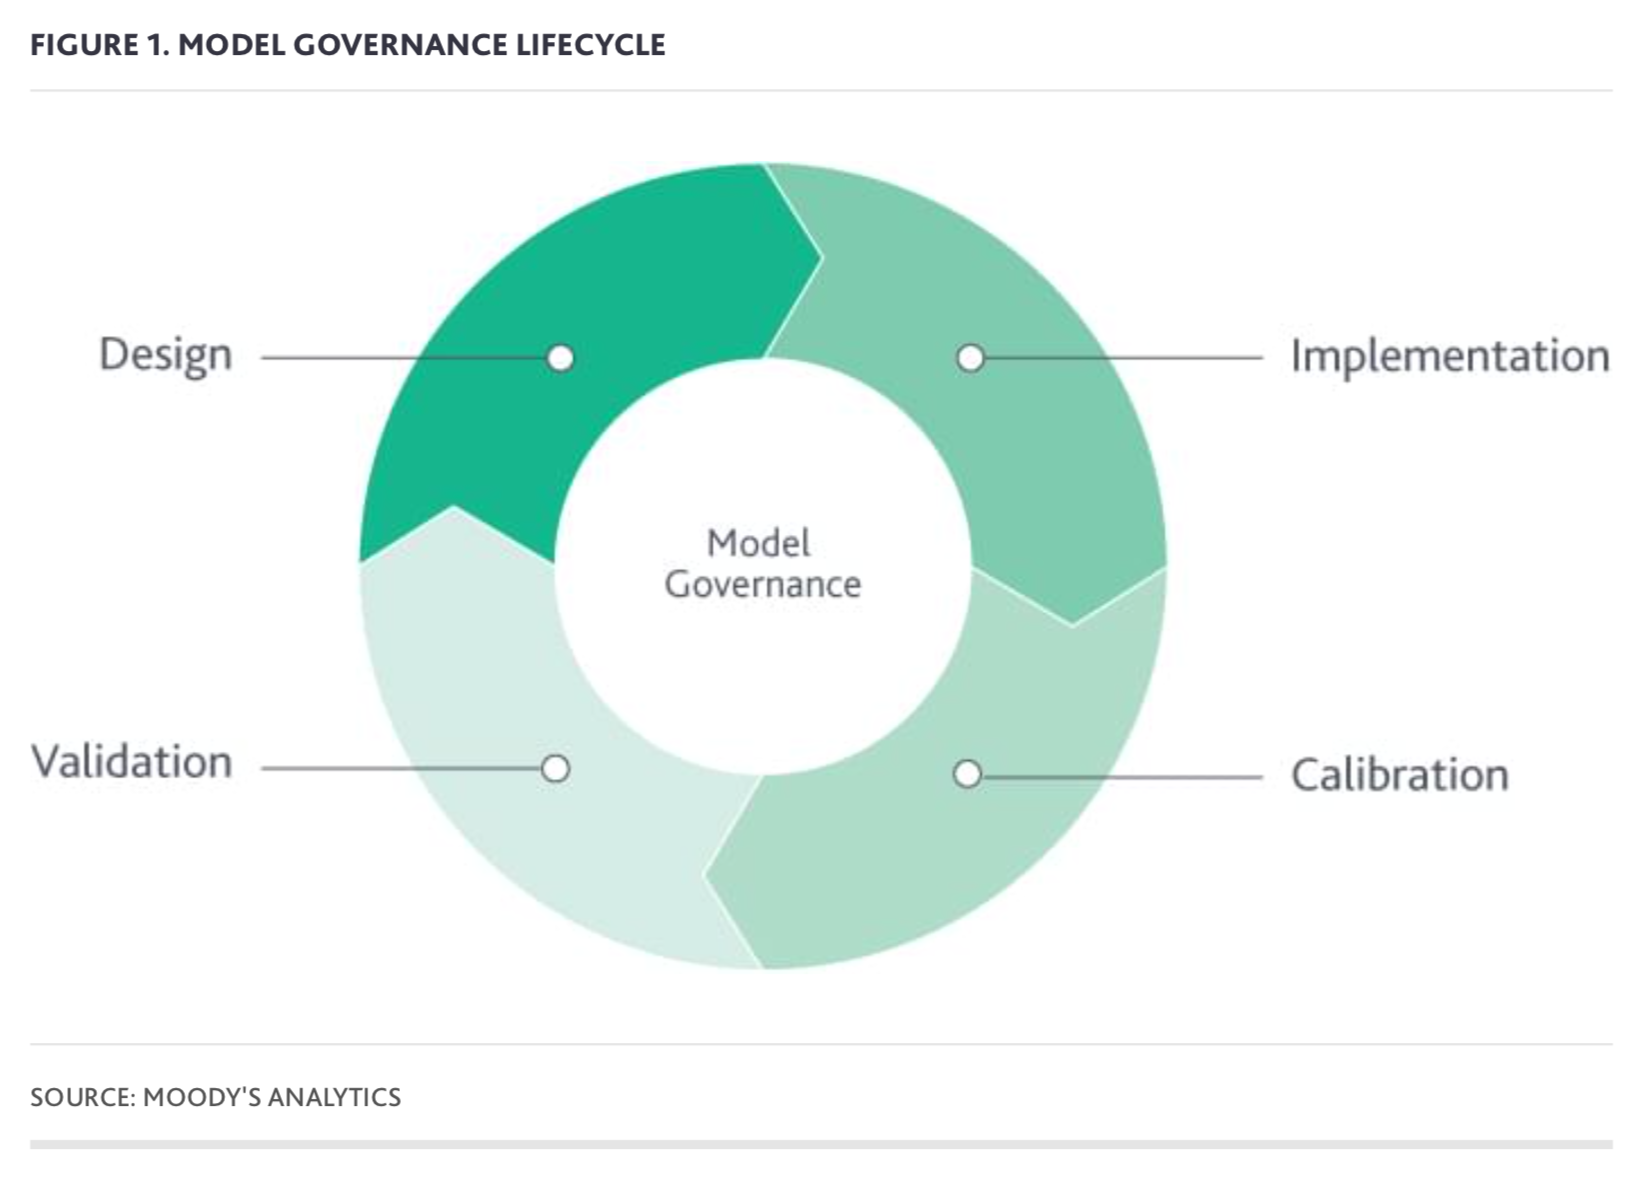
\includegraphics[scale=.3]{images/model_gov_lifecycle}
\end{figure}
\end{frame}


\begin{frame}
\frametitle{Model governance lifecycle vs model development lifecycle}
\begin{figure}[h]
	\centering
	\subfloat[Governance]{{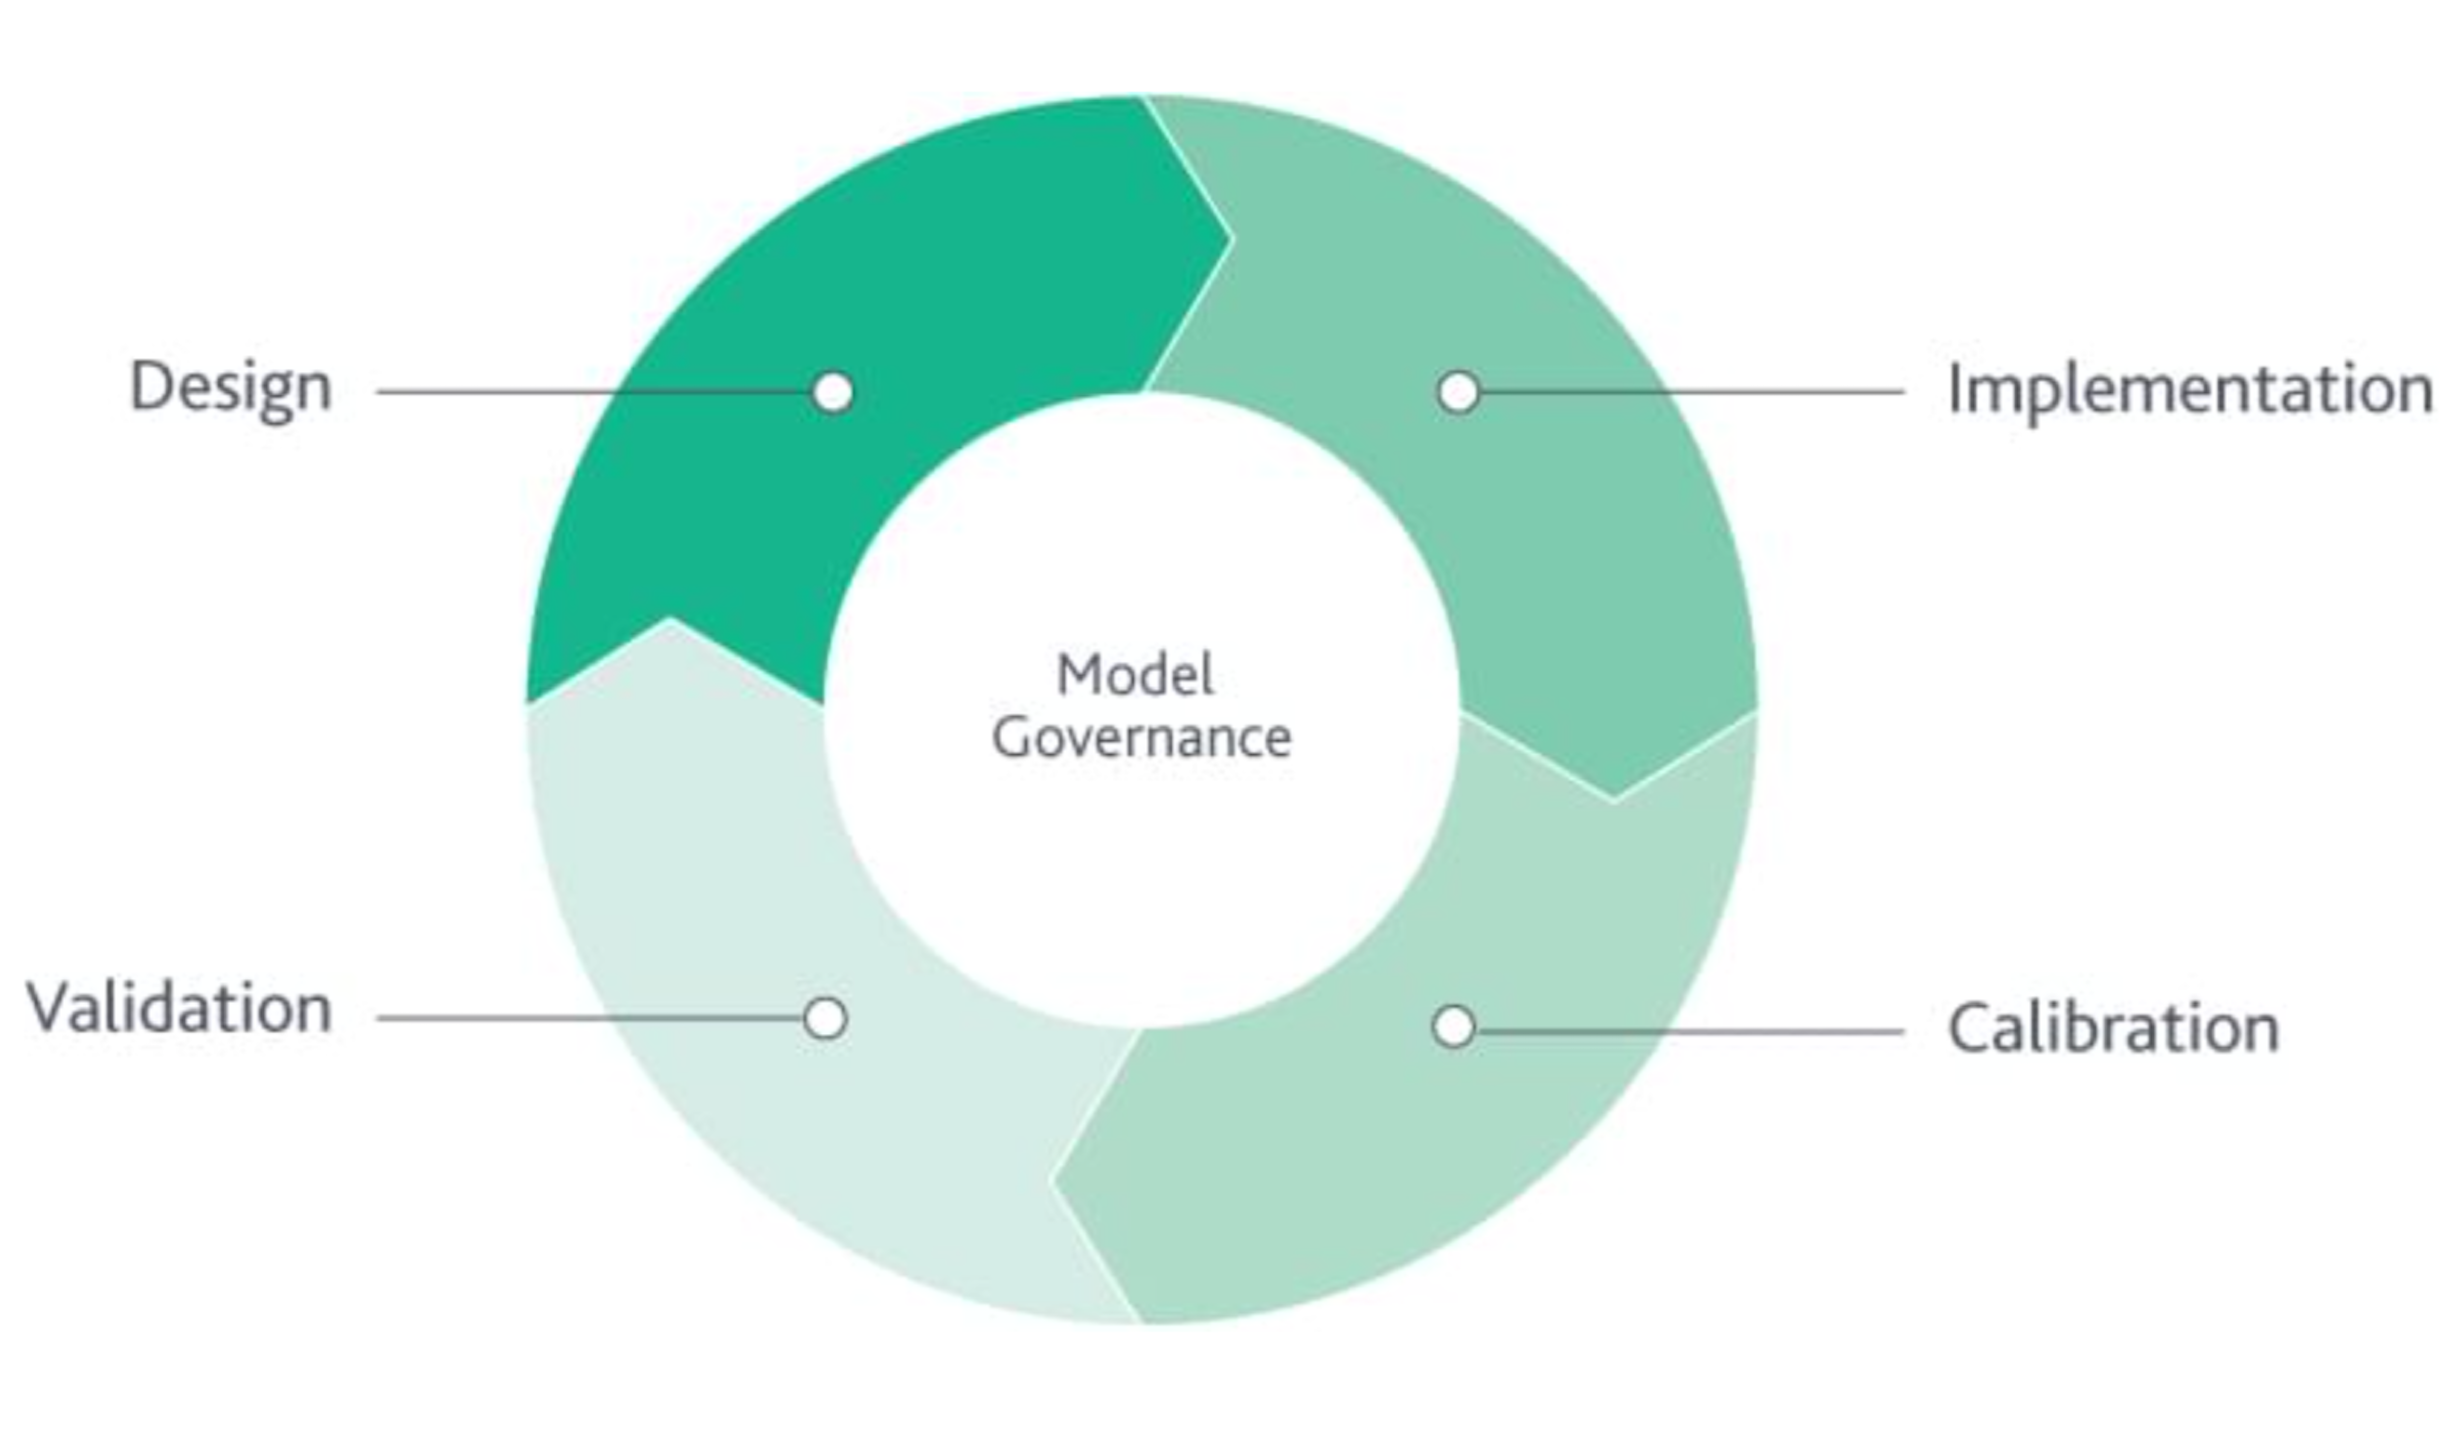
\includegraphics[width=5cm, height=7cm]{images/model_governance_lifecycle2} }}%
	\qquad
	\subfloat[Development]{{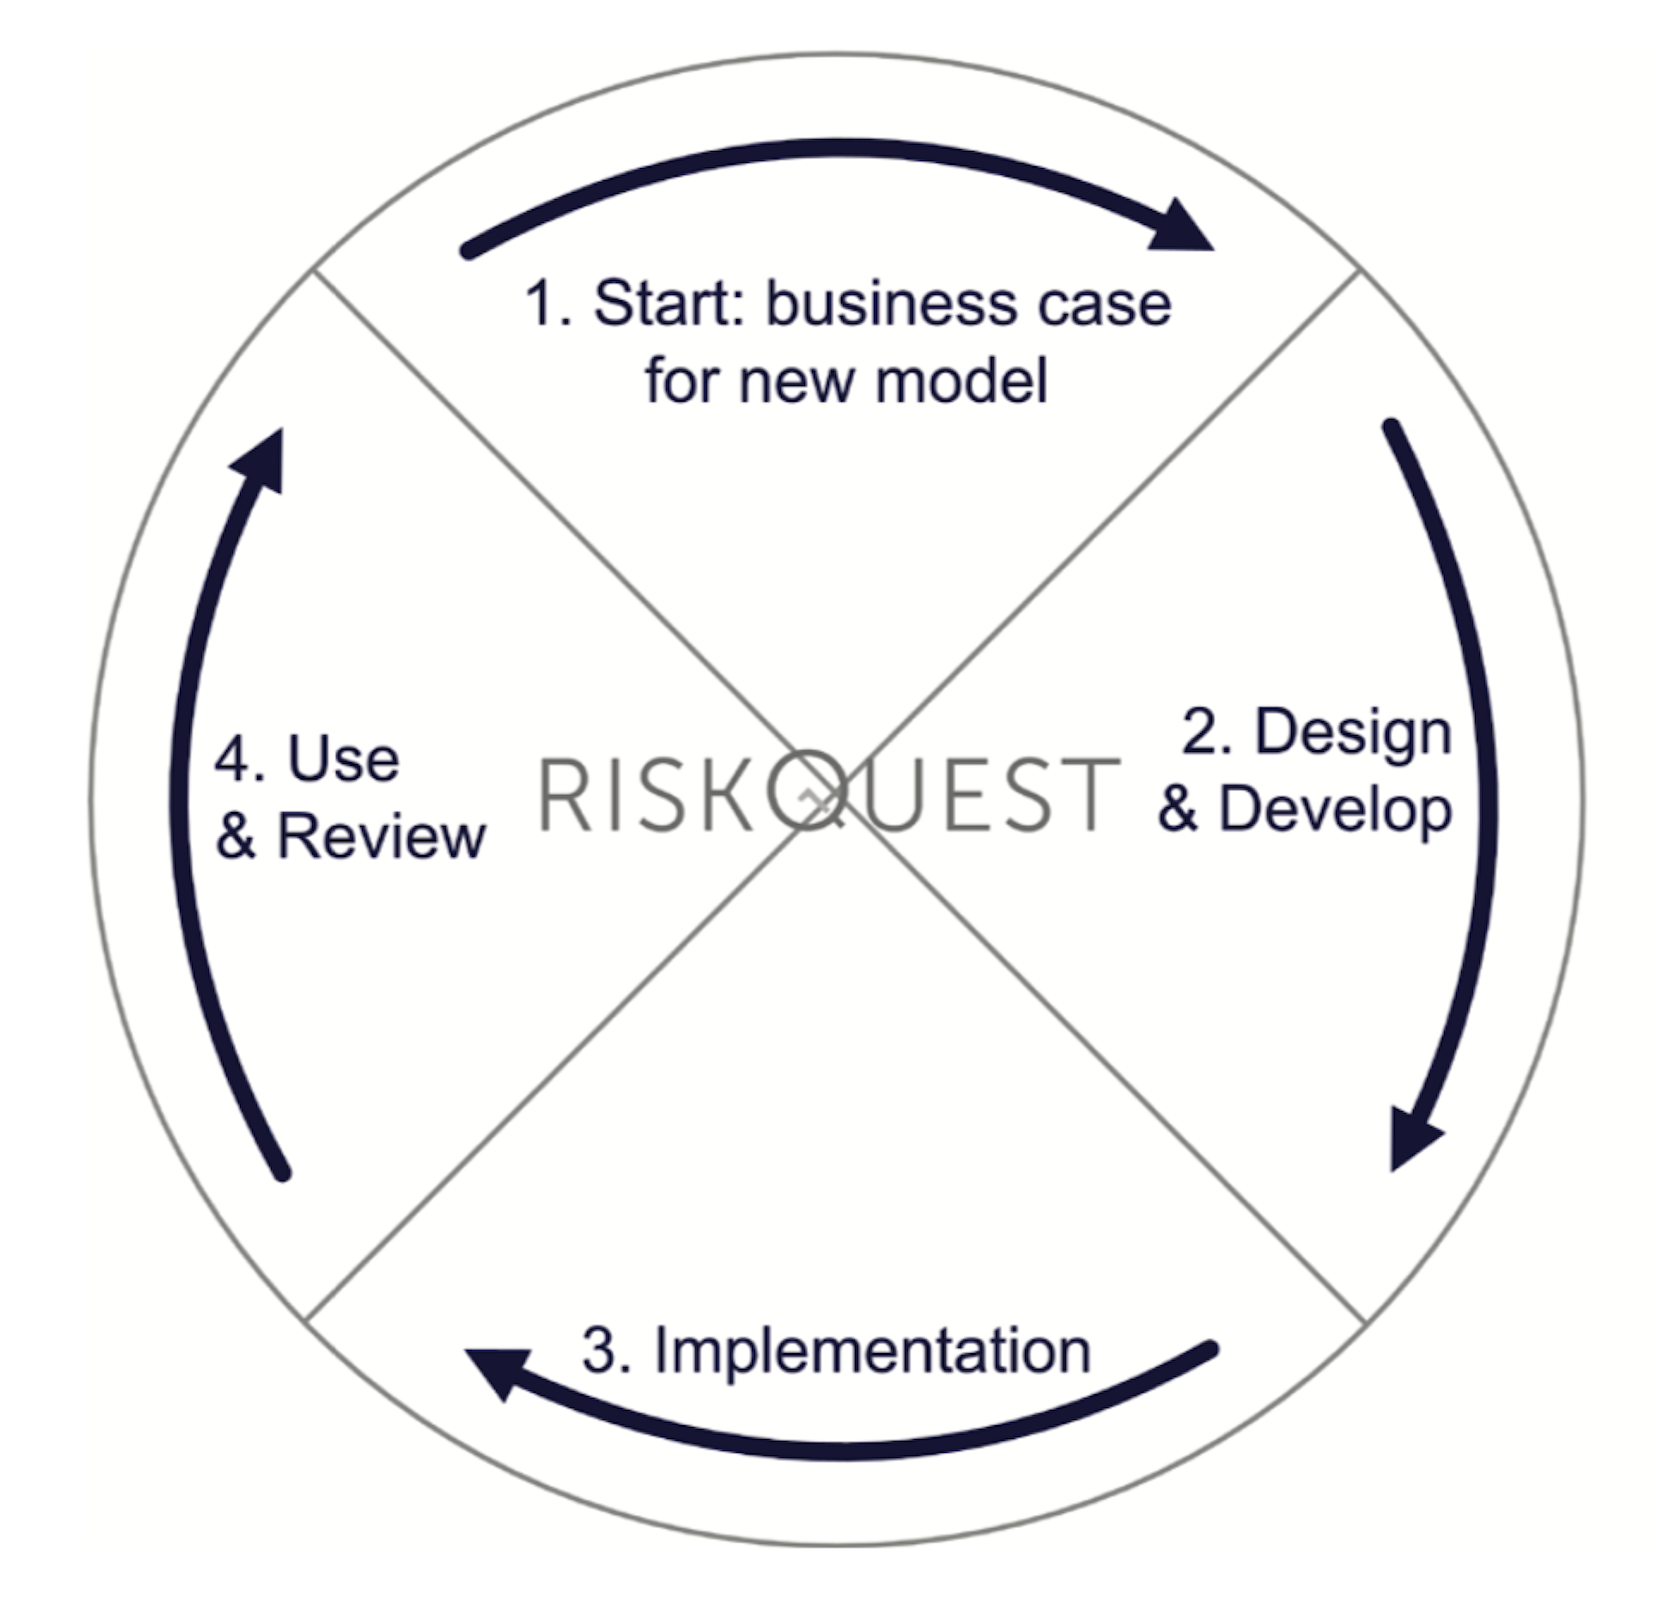
\includegraphics[width=5cm, height=7cm]{images/model_lifecycle2} }}%
\end{figure}
\end{frame}


\begin{frame}
\frametitle{Model governance lifecycle}
Overall governance set around a model’s lifecycle
\begin{itemize}
\item model development (design)
\item model implementation
\item model calibration
\item model validation
\end{itemize} 
\end{frame}


\begin{frame}
\frametitle{Model risk governance framework}
\begin{figure}[h]
	\centering
	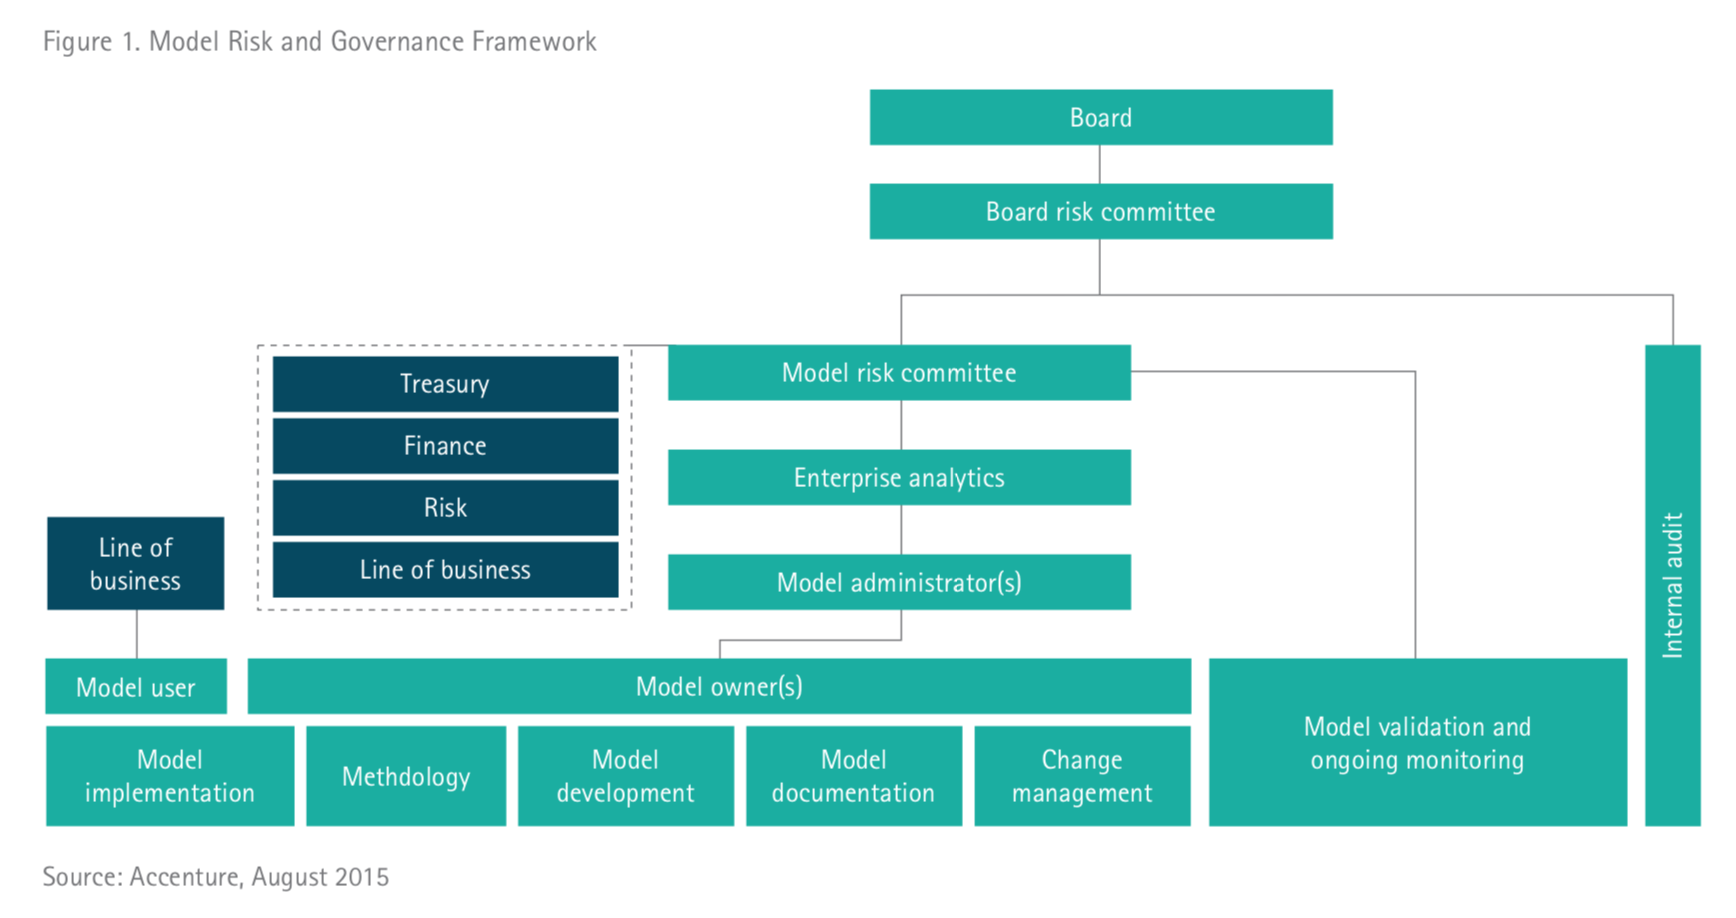
\includegraphics[scale=.35]{images/model_risk_gov_framework}
\end{figure}
\end{frame}


\begin{frame}
\frametitle{Model governance: 3 lines of defense}
\begin{figure}[h]
\centering
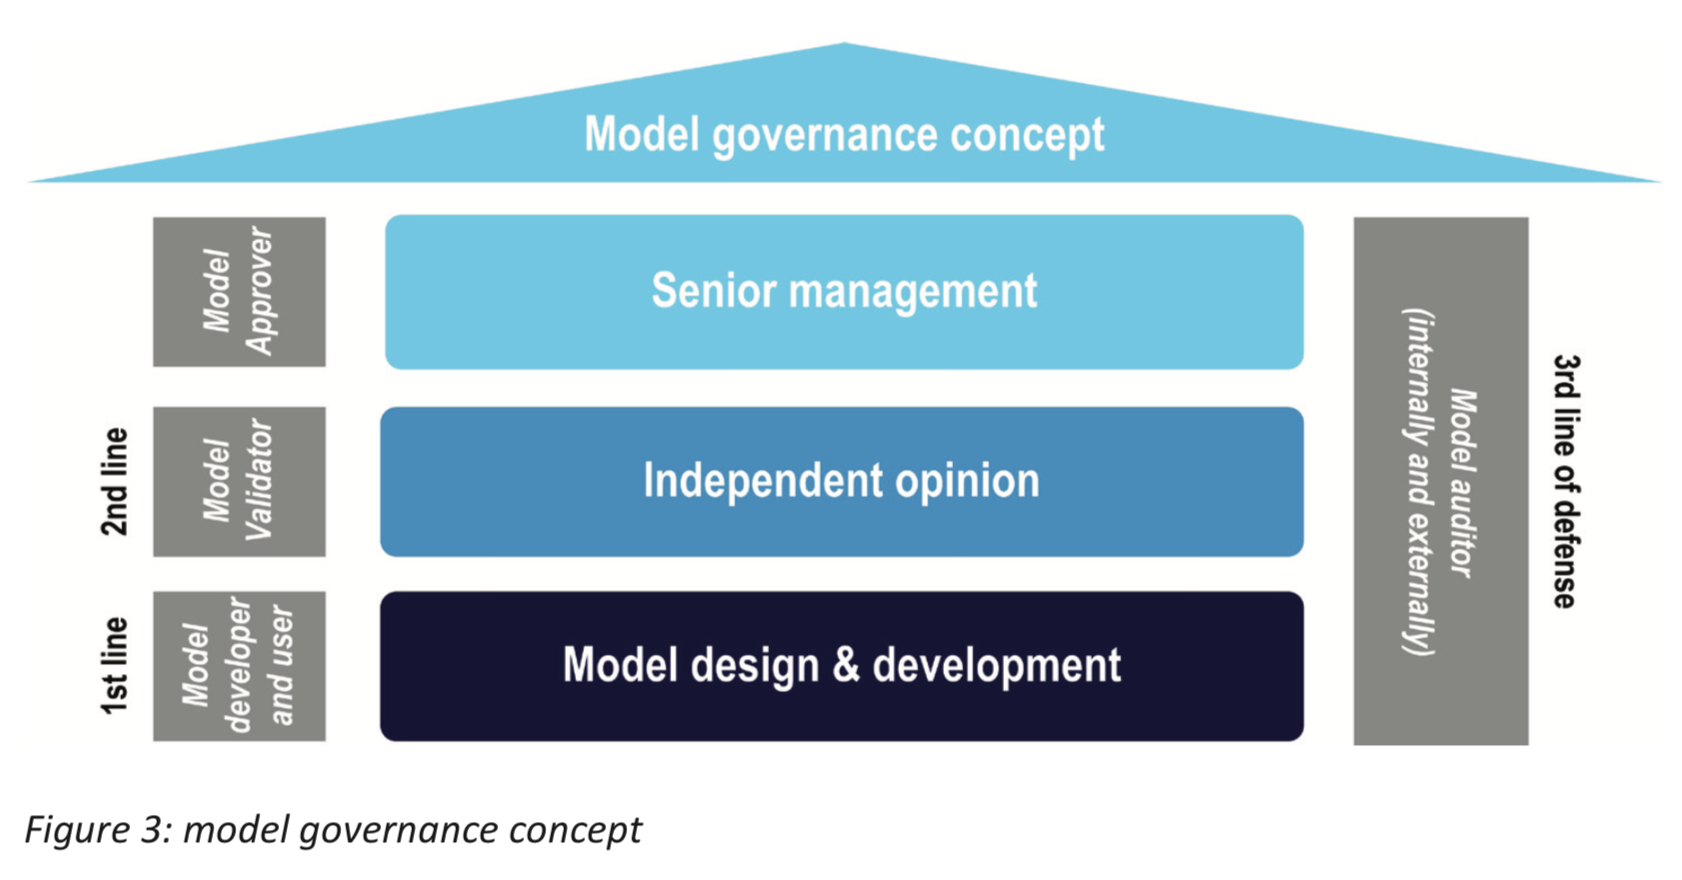
\includegraphics[scale=.3]{images/3_lines_of_defense}
\end{figure}
\end{frame}

%
%\begin{frame}
%\frametitle{Audit review framework}
%\begin{figure}[h]
%	\centering
%	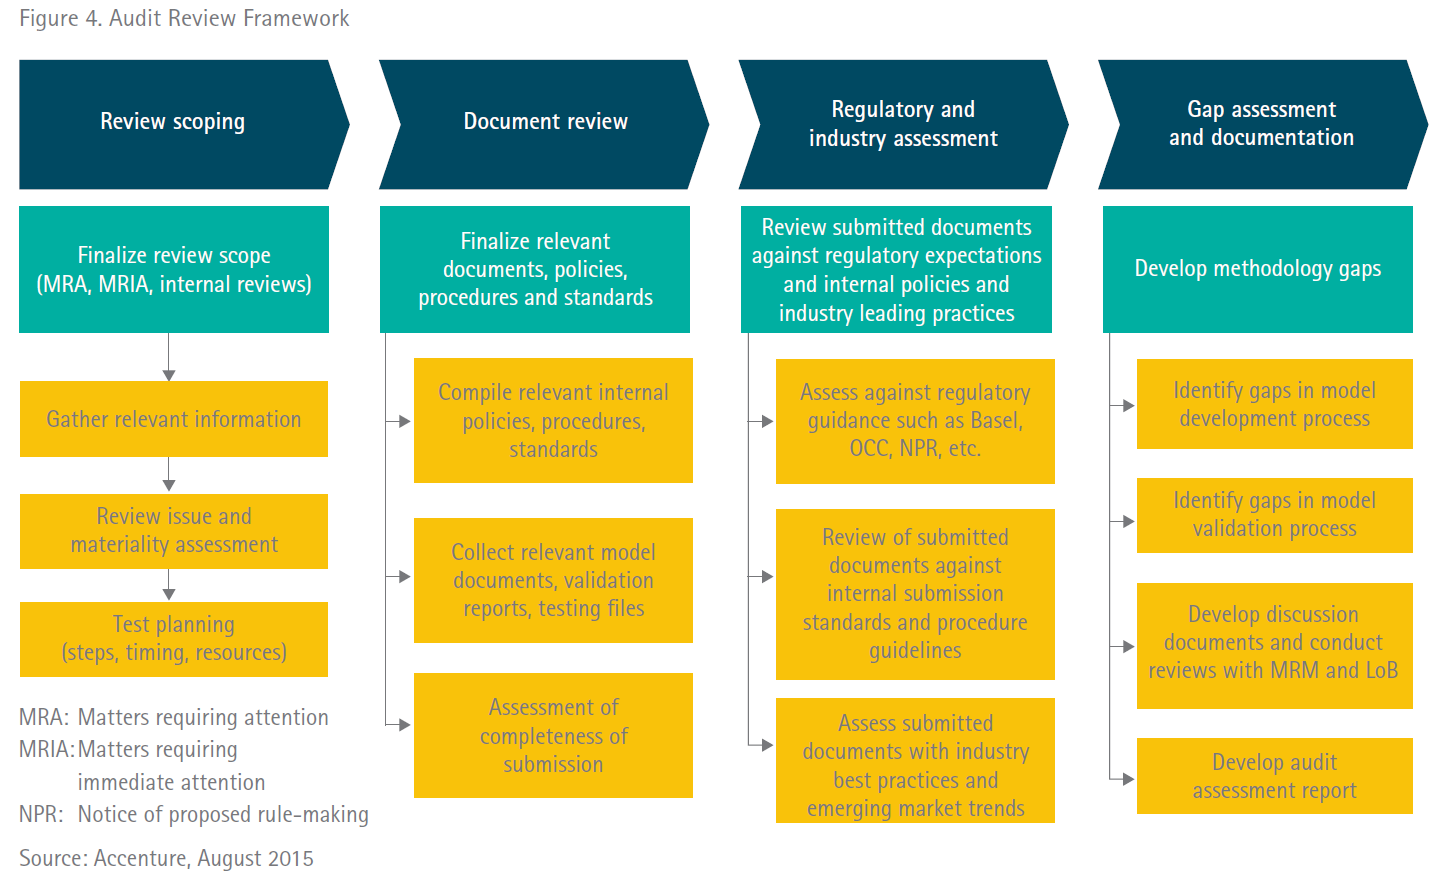
\includegraphics[scale=.3]{images/gov3}
%\end{figure}
%\end{frame}
%
%
%\begin{frame}
%\frametitle{Board engagement and communication}
%\begin{figure}[h]
%	\centering
%	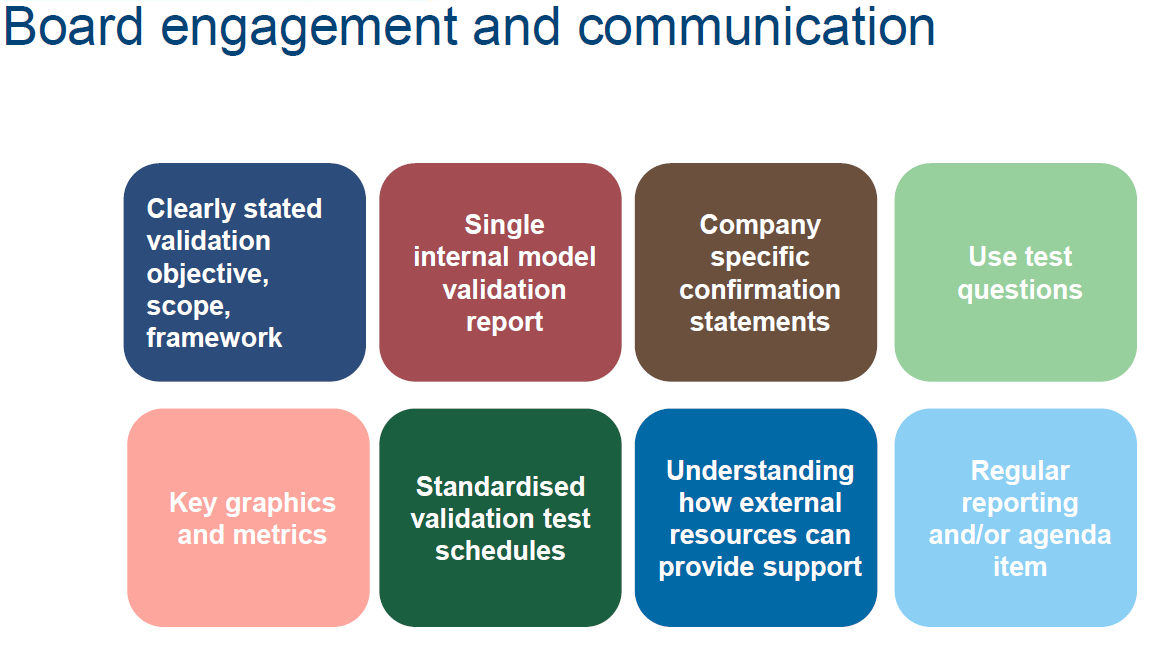
\includegraphics[scale=.3]{images/gov4}
%\end{figure}
%\end{frame}


\begin{frame}
\frametitle{8 key elements for a solid model governance framework}
\begin{figure}[h]
	\centering
	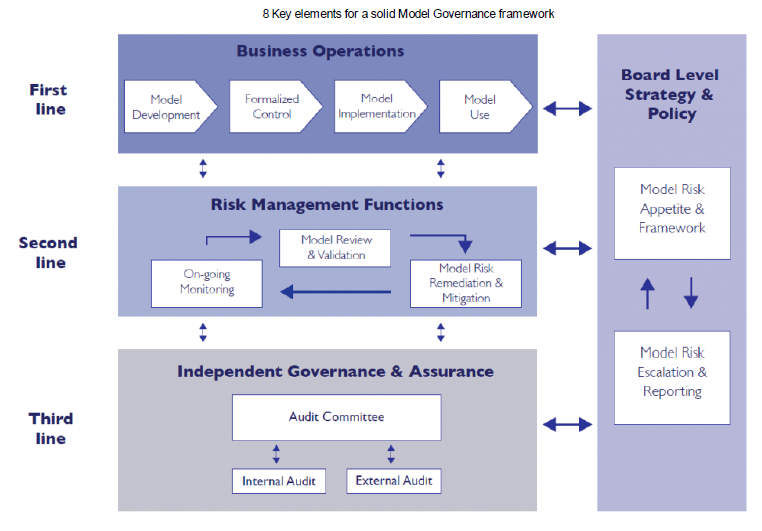
\includegraphics[scale=.5]{images/gov1}
\end{figure}
\end{frame}


\begin{frame}
\frametitle{8 key elements for a solid model governance framework}
\begin{itemize}
\item Development %- Management of model risk begins from the development. The most important elements involved in the process (such as the developers that lead the components in the model definition with their experience) work here. The written documentation that describes every step of the process becomes essential for the quick and easy identification of the different correct phases.
\item Validation %- It is consider as the core phase to test models and classify their solidity. Validation refers to the statistical methodologies used, the input/output information and the performance. From the governance perspective, some important elements to be considered, like where to find all the necessary information or when the validation material is incomplete.
\item Approval %- Critical phases are designing, building and distributing reports to have a complete view of what is Model Governance. It is an essential element for financial institution in order to send reports to the regulators.
\item Modification %- In a common scenario, we can find the absence or the partial presence of documentation, especially for model customization (most of the times, it is identified with an unofficial document). That practice is currently under regulator care, which requires that all the elements related to the model are quick and easy to find.
\item Implementation %- In the stage of implementation, the model is taken over and managed by several departments. The risk here is that some basic components, such as references to origin sources, model execution codes, or technical documents, can be lost. A framework that govern the overall process becomes central in order to avoid that actors involved can perform their activities without a well­identified and configured design.
\item Retirement %- Usually model retirement is undervalued or underestimated, compared to the other phases. However the performance track of models is crucial to take the best decision and to change it when it is not enough efficient.
\item Inventory %- Model inventory is essential to obtain a big picture about what models are currently in place, which are unused, what will be used, etc... It is a synergistic view: looking everything in relation to the models from a single point of view. It allows to track every object linked to models (i.e. documentation, codes, data, etc.) as well as to identify every phase in the model life­cycle (basically, all the elements that contribute in the model risk evaluation).
\item Information sharing %- In a complex process, communication becomes an essential factor for the actors involved; especially when there is a parent­child relationship of dependency in the phases. A Governance framework allows a better information sharing in terms of notification, messages, reports or documents to support and govern the entire process of model life­cycle.
\end{itemize}
\end{frame}


\begin{frame}
\frametitle{Model governance best practices}
\begin{itemize}
	\item model definitions
	\item model inventory
	\item model categorization
	\item model risk teams
\end{itemize}
\end{frame}


%\begin{frame}
%\frametitle{Model monitoring}
%\begin{itemize}
%	\item Model monitoring is the regular analytical review of model performance.
%	\item A robust system of ongoing model monitoring is a key component in the management of model risk.
%	\item Ongoing monitoring is essential to evaluate whether changes in products, exposures, activities, customers or market conditions call for adjustment, redevelopment, or replacement of the model or to verify that any extension of the model beyond its original scope is valid. 
%	\item Any model limitations or assumptions identified in the development stage should be assessed as part of ongoing monitoring.
%	\item In practice, monitoring begins when a model is first implemented in production systems for actual business use. 
%\end{itemize}	
%\end{frame}
%
%
%\begin{frame}
%\frametitle{Model monitoring}
%\begin{itemize}
%	\item This monitoring process should have a frequency appropriate to the nature of the model, the availability of new data or modeling approaches, and the magnitude of the risks involved. 
%	\item This should be clearly laid out as part of a monitoring standards document.
%	\item Model monitoring is an area of increasing importance and regulatory scrutiny as models are treated as critical organizational assets.
%	\item The Federal Reserve has issued guidelines on model monitoring in its SR 11-7 guidance note as well as annual guides on the Comprehensive Capital Analysis and Review (CCAR) process.
%	\item Four similar documents have been issued by the Basel Committee and the Bank of England.
%\end{itemize}
%\end{frame}
%
%
%\begin{frame}
%\frametitle{Model monitoring}
%\begin{itemize}
%	\item A strong model monitoring process has proven to be a potent competitive advantage for those organizations that take extra steps to help ensure the
%	effectiveness of their model monitoring. 
%	\item These steps include:
%	\begin{itemize}
%		\item diligently tracking model performance, 
%		\item escalating and resolving model issues, 
%		\item involving senior management in decision making, 
%		\item fine-tuning models on a timely basis, and 
%		\item maintaining well-documented logs and rationales of changes.
%	\end{itemize} 
%	\item Effective monitoring allows institutions to closely control and better empower the strategic risk management tools for day-to-day operational management.
%\end{itemize}	
%\end{frame}
%
%
%\begin{frame}
%\frametitle{Challenges to model monitoring}
%Processes related to model monitoring may be affected by:
%\begin{itemize}
%	\item Governance: A lack of policies around model risk monitoring, or policies in place may not be properly enforced; %No full model list for audit tracking purposes; or a list not regularly updated.
%	\item Organization: The organization finding itself in reactive mode, often scrambling frantically to meet internal and external deadlines; %Timelines regularly affected by poor capacity planning and inadequate contingency plans.
%	\item Processes and procedures: No standards in place surrounding the frequency of model monitoring; %similar teams using different standards and procedures for model tracking templates or for performance metrics.
%	\item Monitoring output analysis: Poorly performing models remaining in production due to decision making affected by inconsistency in metrics, frequency, lack of analysis of root causes, or by ineffective and poor commentaries on monitoring output.
%	\item Operational risks: Lack of automation, regular controls in code and of tracking logs, leading to a high error rate; %Lack of contingency plans lead to the risk of losing key historical facts if dedicated personnel leave the firm and adequate logs are not in place.
%\end{itemize}
%\end{frame}
%
%
%\begin{frame}
%\frametitle{Key principles of effective model monitoring}
%\begin{itemize}
%	\item Enterprise level model inventory
%	\item Robust data monitoring processes
%	\item Governance structure
%	\item Comprehensive indicators for model performance
%	\item Model discrimination
%	\item System stability
%	\item Characteristic stability
%	\item ‘Actual versus expected’ or calibration
%	\item Scoring analysis distribution
%	\item Override analysis
%\end{itemize}
%\end{frame}


%\begin{frame}
%\centering
%Model inventory, enterprise level model inventory, complexity
%\end{frame}

%\begin{frame}§
%\frametitle{Enterprise level model inventory}
%\begin{figure}[h]
%	\centering
%	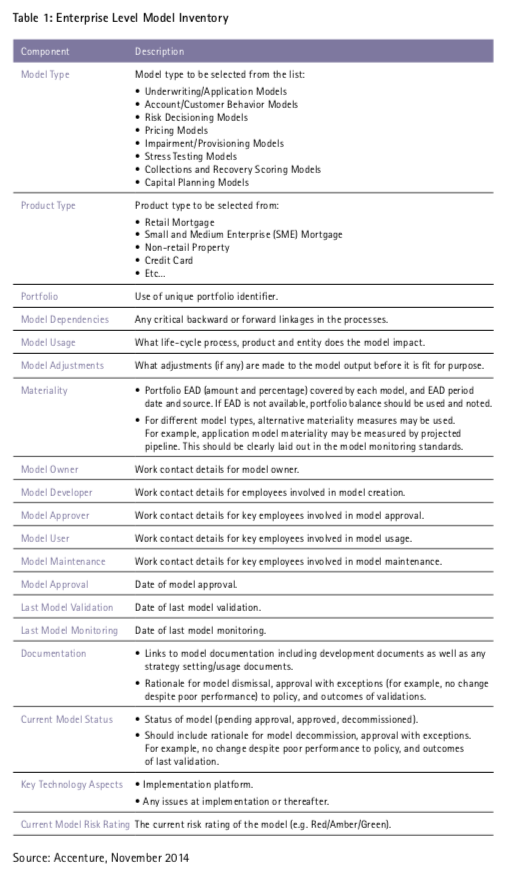
\includegraphics[scale=.5]{images/enterprise_level_model_inventory}
%\end{figure}
%\end{frame}

%\begin{frame}
%\frametitle{Model governance/management process}
%The model governance process intends to appropriately define the role of each model stakeholder during each phase of the model life cycle.
%\begin{itemize}
%	\item model owner
%	% Typically the business that requests the model (re)design and that is the main user of the model. The model owner sets the business requirements for the mod- el, is responsible for user acceptance testing and ensures a correct roll out of the model to the users (e.g. training, communication, etcetera).
%	\item model developer
%	% The Model Developer develops, tests and documents the model in accordance with the regulatory requirements and the business requirements set by the model owner. In addition, the Model Developer is responsible for reviewing the model.
%	\item model validator
%	% The Model Validator provides an independent validation of the model. To ensure its independence the model validator abstains from any participation in the model development process. The aim of the validation process is to determine whether a model is (still) appropriate for its use or intended use (“fit for purpose”).
%	\item model approver
%	% All models must be approved by the Model Approver prior to implementation.
%	\item model users
%	% The Model Users use the model outputs in their day-to-day operations. In general, the business that requests the model (re)development and that is the main user of the model.
%	\item model auditor
%	% The Model Auditor performs audits of the model management process. In addition, the Model Auditor may perform special audits in accordance with its audit plan.
%	\item model implementer
%	% All models are implemented. This can either be done within the IT infrastructure (preferred way) or stand alone (e.g. in a local spreadsheet).
%\end{itemize}
%The minimum information required per model consists of
%\begin{itemize}
%	\item Model name (model identification), type and location,
%	\item Model owner (name and function),
%	\item Model type,
%	\item Modeling environment: type of systems used,
%	\item Descriptive characteristics: model uses and/or purposes.
%\end{itemize}
%The model inventory will be reviewed periodically. All model changes are to be reflected.
%The inventory should cover at a minimum:
%\begin{itemize}
%	\item Intended and approved use of the model %(e.g., which instruments it covers, what types of measures can be calculated using this model, etc.)
%	\item Last calibration date and calibration frequency
%	\item Validation status %(passed, failed, passed with caveats)
%	\item Date of model sign ­off and level of sign ­off
%	\item Link to relevant documentation and date of latest documentation review 
%	\item Significant manual overrides and their justification
%	\item Other known issues
%	\item Dependencies on other models/modules
%\end{itemize}
%\end{frame}
%
%
%\begin{frame}
%\frametitle{Model categorization}
%\begin{itemize}
%	\item In order to manage the risk associated with the use of models, firms can also separate them in different groups by their complexity (both theoretical and implementation) and materiality, measured by the impact that their use (or misuse) may have on the firm.
%	\item These categorizations will also inform the frequency of the calibration and validation needed for the different models.
%	\item They will also inform banks of the intended and correct use of a model and help them decide whether its use can be extended to other purposes or instruments without a thorough review by the model developers, recalibration, and/or revalidation.
%\end{itemize}
%\end{frame}

%\begin{frame}
%\frametitle{Enterprise level model inventory}
%\begin{itemize}
%	\item A model inventory takes stock of the models used by an institution and establishes clear ownership of the maintenance and usage of the model. 
%	\item Some measure of the materiality of the model or portfolio should be included %(common measures include the portfolio balance or exposure at default).
%	\item Guidelines for establishing a model inventory
%	\begin{itemize}
%		\item Segregate the inventory building exercise by model category.
%		\item Within each category, maintain a complete listing of all models used across the entity or group of entities.
%		\item The inventory should be careful to also include any sub-models or ‘feeder’ models.
%	\end{itemize}
%\end{itemize}
%\end{frame}
%
%
%\begin{frame}
%\frametitle{Robust data monitoring processes}
%\begin{itemize}
%	\item Models are data intensive by their nature and typically are designed to accept inputs from underwriting/origination systems, transaction processing systems, core banking systems and other sources.
%	\item Errors in raw data or in model variables may be reflected in model monitoring reports, but often happens too late to prevent negative effects on the business. 
%	\item To avoid such problems, data quality and consistency rules should be considered and created for each raw data field to help ensure the integrity of the data dimensions feeding the model.
%	\item A best practice common to a number of large banking institutions is to establish a data monitoring process that precedes model monitoring
%\end{itemize}
%\end{frame}
%
%
%\begin{frame}
%\frametitle{Robust data monitoring processes}
%A large European bank has a monthly process to help run all model input data through a validation engine with approximately 8,000 rules. The engine analyzes the model input file and generates a monthly model data quality report, indicating the variable(s) affected and models affected, if any.
%\end{frame}
%
%
%\begin{frame}
%\frametitle{Robust data monitoring processes}
%\begin{figure}[h]
%	\centering
%	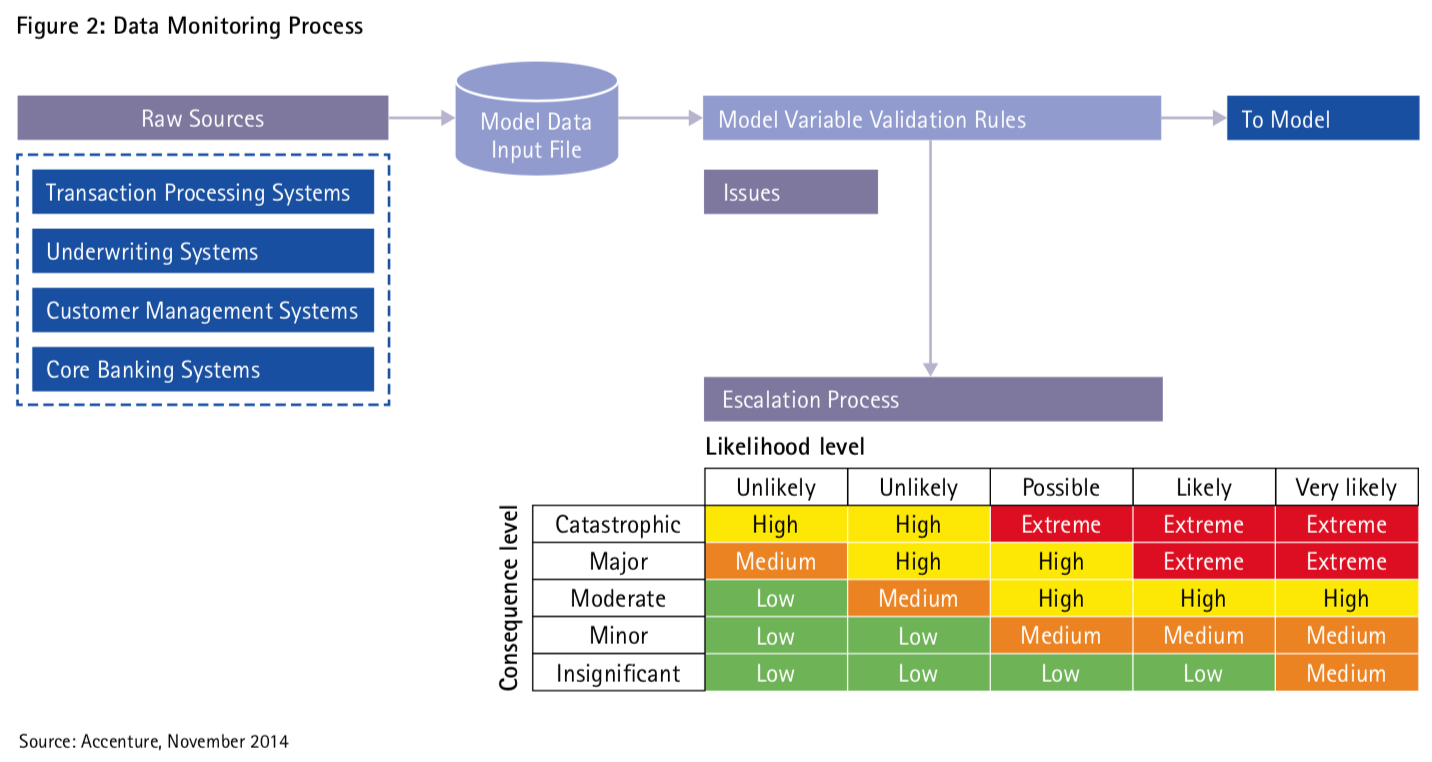
\includegraphics[scale=.22]{images/data_monitoring_process}
%\end{figure}
%\end{frame}
%
%
%\begin{frame}
%\frametitle{Governance structure}
%\begin{figure}[h]
%	\centering
%	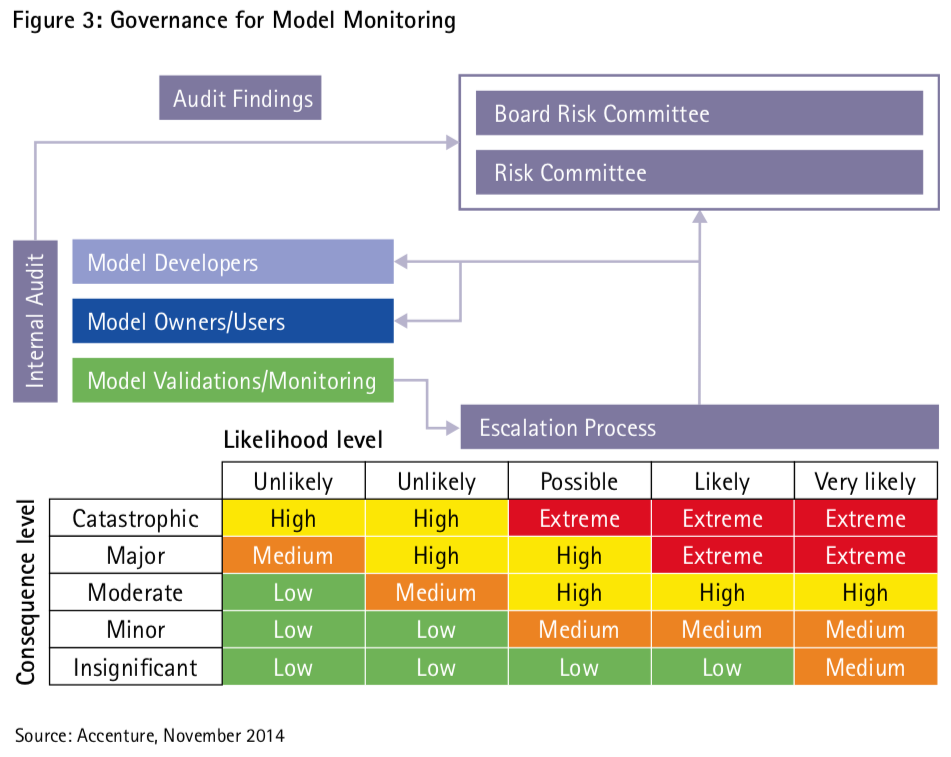
\includegraphics[scale=.3]{images/governance_for_model_monitoring}
%\end{figure}
%\end{frame}
%
%
%\begin{frame}
%\frametitle{Critical components of a robust governance structure}
%\begin{itemize}
%	\item Independence of the model monitoring team from the model development team;
%	\item Effective model audit processes and procedures; and
%	\item Engagement and involvement from senior management.
%\end{itemize}
%It is important to have communication across all three lines of defense.
%\end{frame}
%
%
%\begin{frame}
%\frametitle{Comprehensive indicators for model performance}
%In practice, it is often observed that organizations adhere to a few simple metrics (notably the Kolmogorov-Smirnov (KS) Statistic, and the Gini Coefficient) for regular monitoring purposes, leaving the more comprehensive checks and related metrics for periodic (often annual, if not bi-annual) validation exercises.
%
%A key best practice employed in conjunction with various performance criteria is the definition of performance thresholds (often called ‘Traffic Lights’) for various metrics. While industry standards are available for certain metrics, most banks would determine acceptable thresholds internally, subject to regulatory supervision.
%\end{frame}
%
%
%\begin{frame}
%\frametitle{Comprehensive indicators for model performance}
%\begin{figure}[h]
%	\centering
%	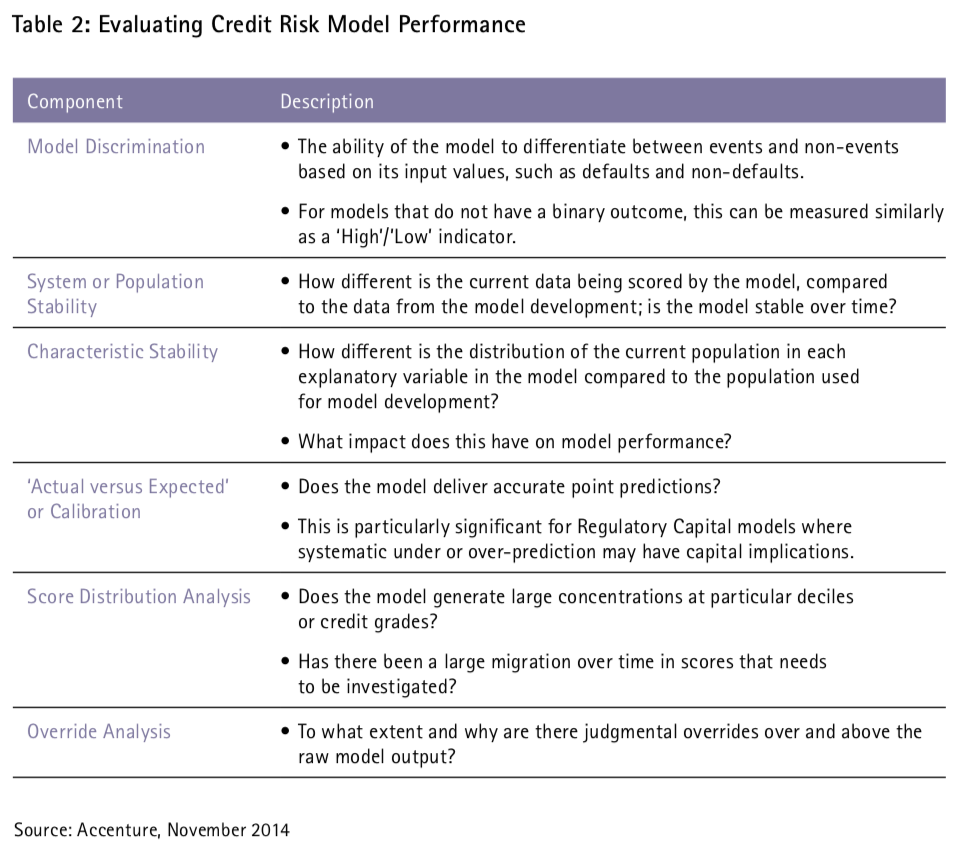
\includegraphics[scale=.25]{images/evaluating_model_performance}
%\end{figure}
%\end{frame}
%
%
%\begin{frame}
%\frametitle{Model discrimination}
%\begin{itemize}
%	\item The measurement of a classification tool’s ability to assess an obligor for the future status is commonly called discrimination.
%	\item The concept is also applicable to models that predict continuous variables in terms of the model’s ability to differentiate between high and low values.
%	\item The KS Statistic and Gini Coefficient	are the two most frequently used metrics in an industry context; in banking, the Basel Committee recommends the Gini Coefficient or accuracy ratio (AR) and the area under curve (AUC) measures.
%\end{itemize}
%\end{frame}
%
%
%\begin{frame}
%\frametitle{Model discrimination}
%\begin{figure}[h]
%	\centering
%	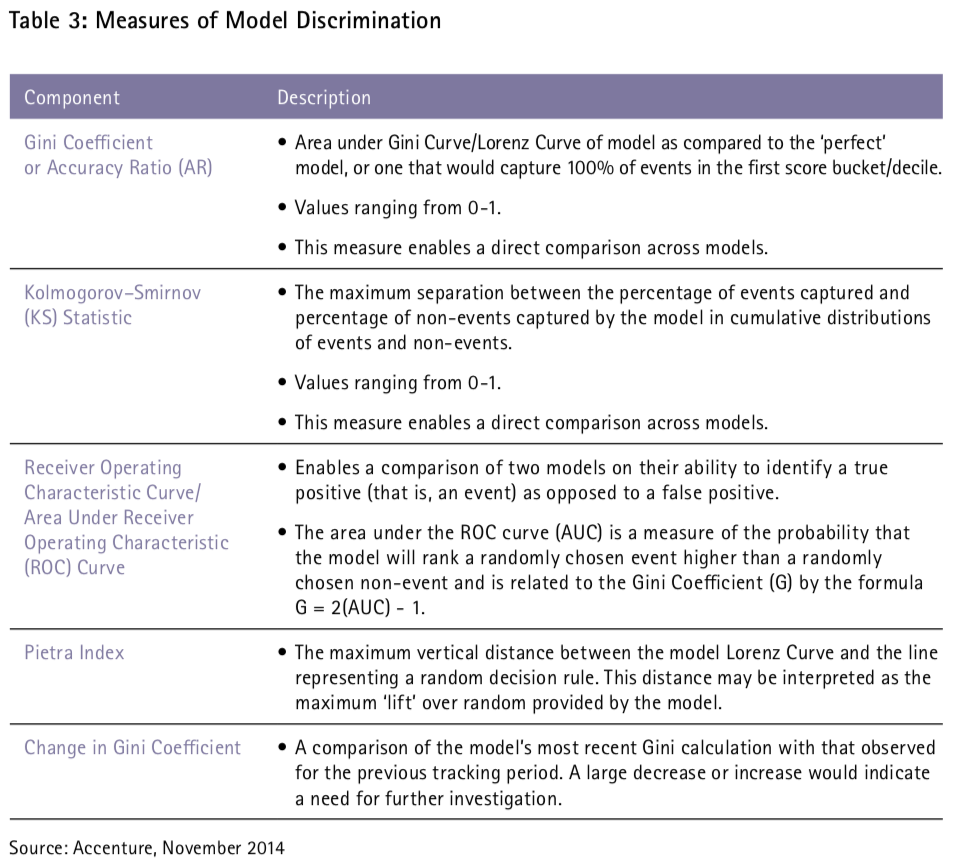
\includegraphics[scale=.25]{images/measures_of_model_discrimination}
%\end{figure}
%\end{frame}
%
% 
%\begin{frame}
%\frametitle{System stability}
%\begin{itemize}
%	\item System stability or population stability compares the data sample the model was developed on with a more recent data sample on which the model has been used. 
%	\item The discriminatory power of a model is based on information contained in the development dataset, and hence large variances from this may cause model performance to deteriorate, or make the model unfit for purpose.
%	\item The Population Stability Index (PSI) is the standard measure for system stability and is also recommended by most regulatory bodies. The PSI is also applicable to models that predict continuous outcomes.
%	\item The transition matrix is critical to PD models and is in most cases a required submission to regulators. Thresholds for the degree of transition that is deemed acceptable are usually set internally by the institution.
%\end{itemize}
%\end{frame}
%
%
%\begin{frame}
%\frametitle{Evaluating system stability}
%\begin{figure}[h]
%	\centering
%	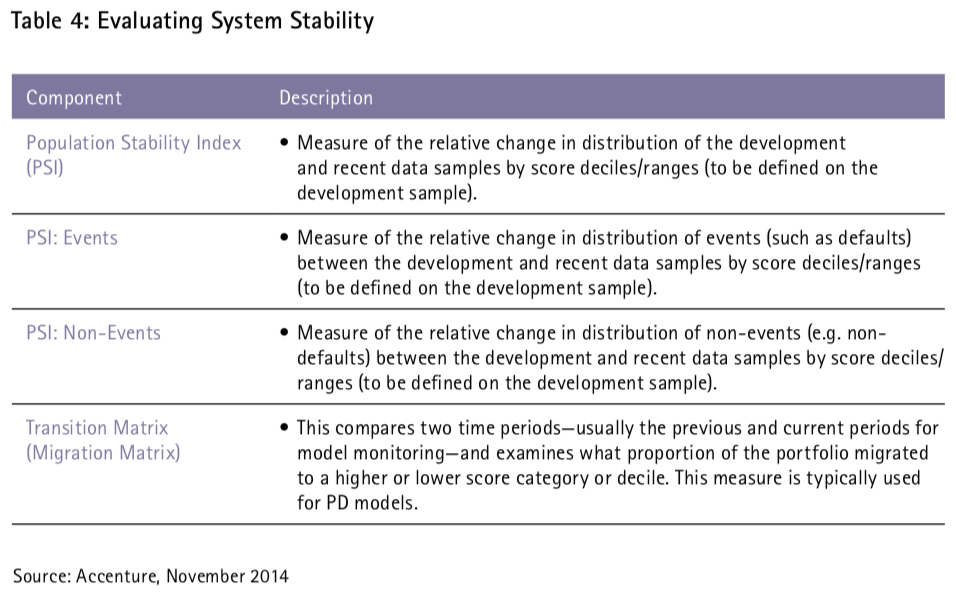
\includegraphics[scale=.3]{images/system_stability}
%\end{figure}
%\end{frame}
%
%
%\begin{frame}
%\frametitle{Characteristic stability}
%\begin{itemize}
%	\item The system stability measures examine a model as a whole but do not examine how individual model characteristics or variables may have changed in distribution during two time periods.
%	\item Characteristic stability measures are increasingly requested by regulators and external auditors as evidence of the thoroughness of a model monitoring system, in addition to the PSI measures.
%\end{itemize}
%\end{frame}
%
%
%\begin{frame}
%\frametitle{Characteristic stability}
%\begin{figure}[h]
%\centering
%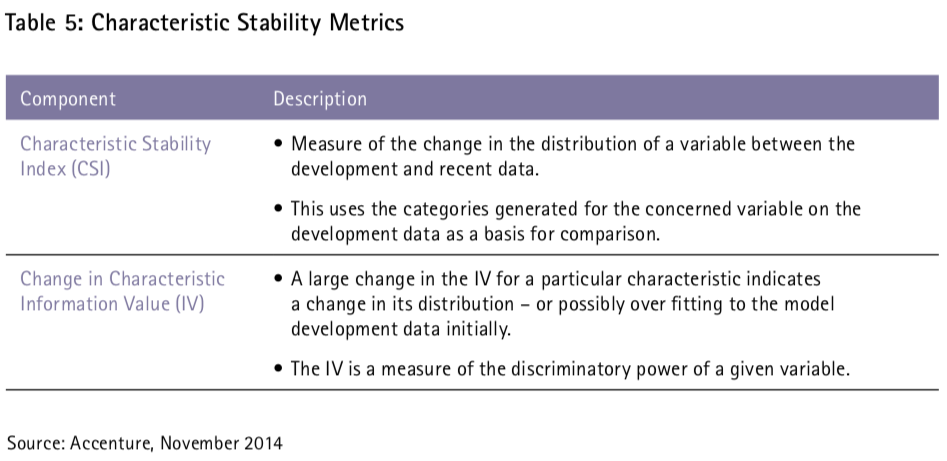
\includegraphics[scale=.3]{images/characteristic_stability_metrics}
%\end{figure}
%\end{frame}
%
%
%\begin{frame}
%\frametitle{‘Actual versus expected’ or calibration}
%\begin{itemize}
%	\item The calibration or actual versus expected performance of a model refers to its ability to yield an accurate point prediction for the output variable.
%\end{itemize}
%\end{frame}
%
%
%\begin{frame}
%\frametitle{‘Actual versus expected’ or calibration}
%\begin{figure}[h]
%\centering
%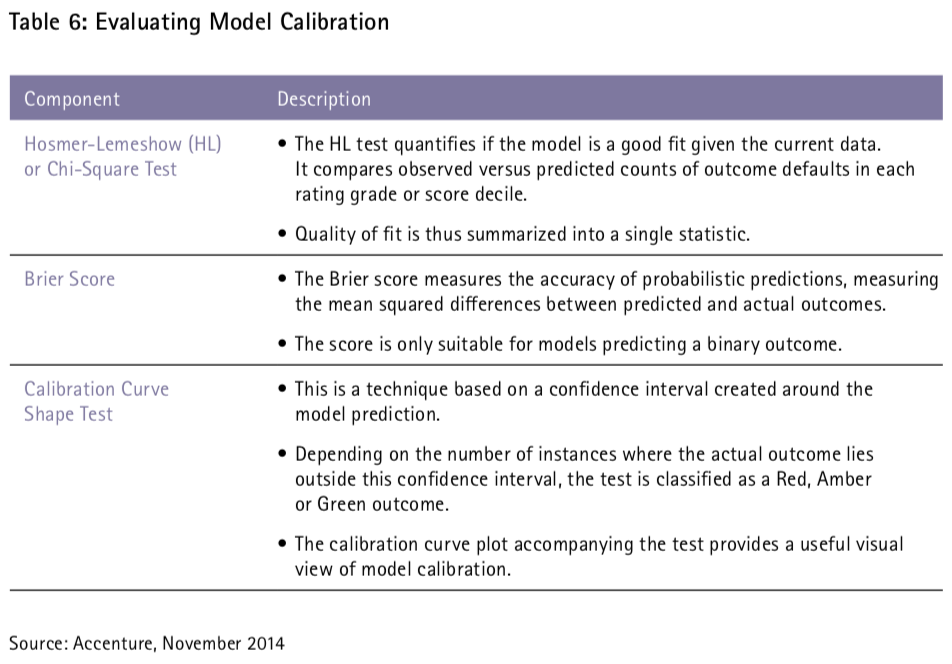
\includegraphics[scale=.3]{images/model_calibration}
%\end{figure}
%\end{frame}
%
%
%\begin{frame}
%\frametitle{Scoring analysis distribution}
%\begin{itemize}
%	\item Models which produce large concentrations in particular credit grades or scores can be problematic, and undesirable from a regulatory perspective.
%	\item The concentration of the score can be measured by the Herfindahl-Hirschman Index.
%\end{itemize}
%\end{frame}
%
%
%\begin{frame}
%\frametitle{Scoring analysis distribution}
%\begin{itemize}
%	\item What level of managerial or other overlays are in place over and above the raw model results.
%	\item An override is defined as having occurred whenever the model output has been ignored or amended.
%\end{itemize}
%\end{frame}
%
%
%\begin{frame}
%\frametitle{Scoring analysis distribution}
%\begin{figure}[h]
%\centering
%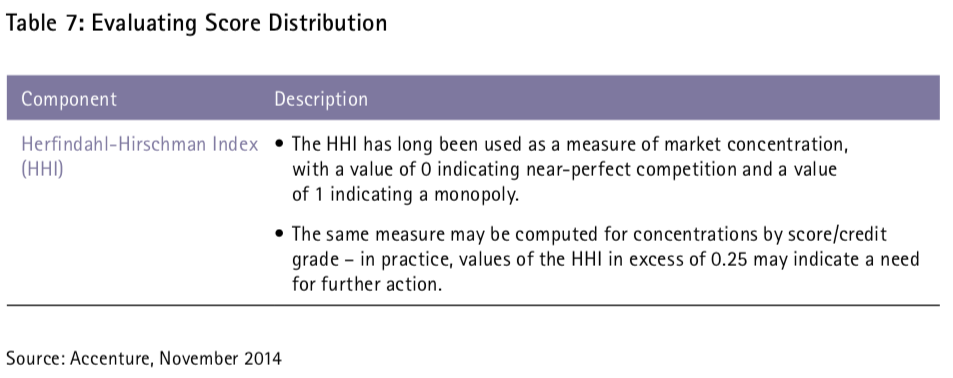
\includegraphics[scale=.3]{images/score_distribution}
%\end{figure}
%\end{frame}
%
%
%\begin{frame}
%\frametitle{Override analysis}
%\begin{figure}[h]
%\centering
%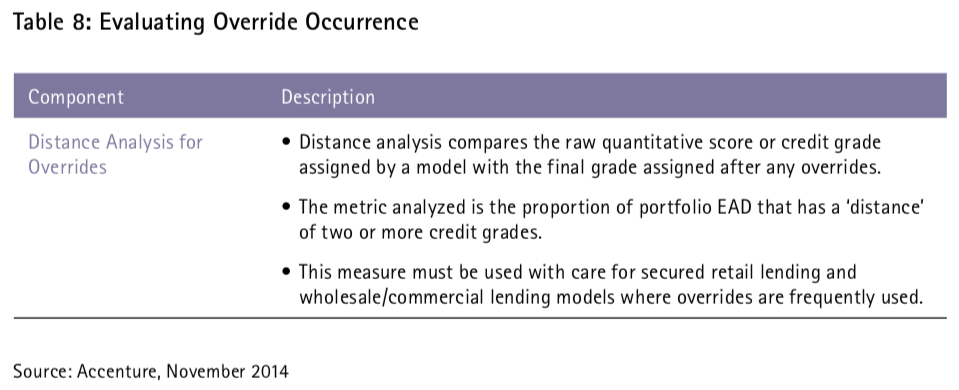
\includegraphics[scale=.3]{images/override_occurrence}
%\end{figure}
%\end{frame}
%
%
%\begin{frame}
%\frametitle{Effective management information systems (MIS)}
%\begin{figure}[h]
%	\centering
%	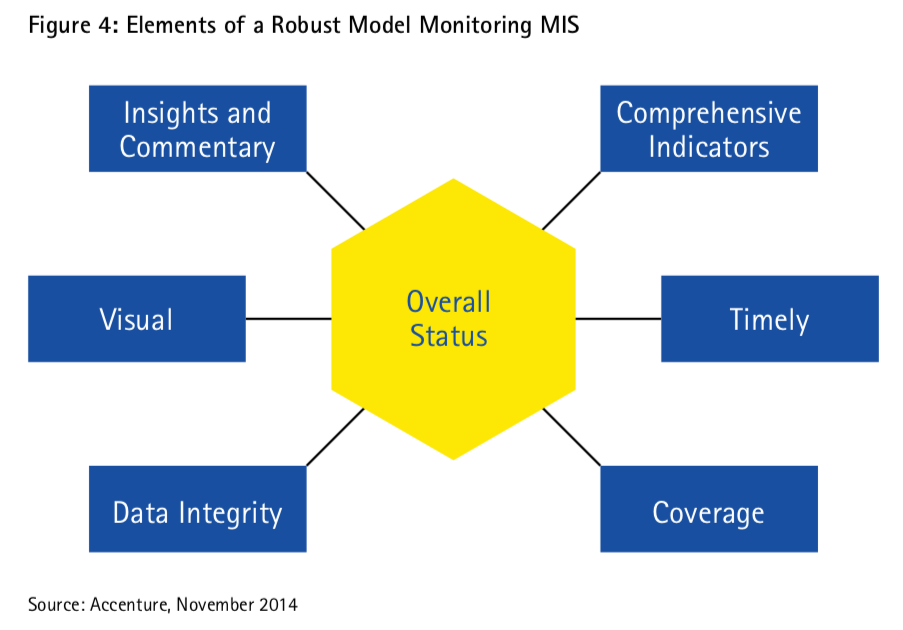
\includegraphics[scale=.3]{images/robust_model_monitoring_mis}
%\end{figure}
%\end{frame}
%
%
%\begin{frame}
%\frametitle{Credit risk model monitoring suite}
%\begin{figure}[h]
%	\centering
%	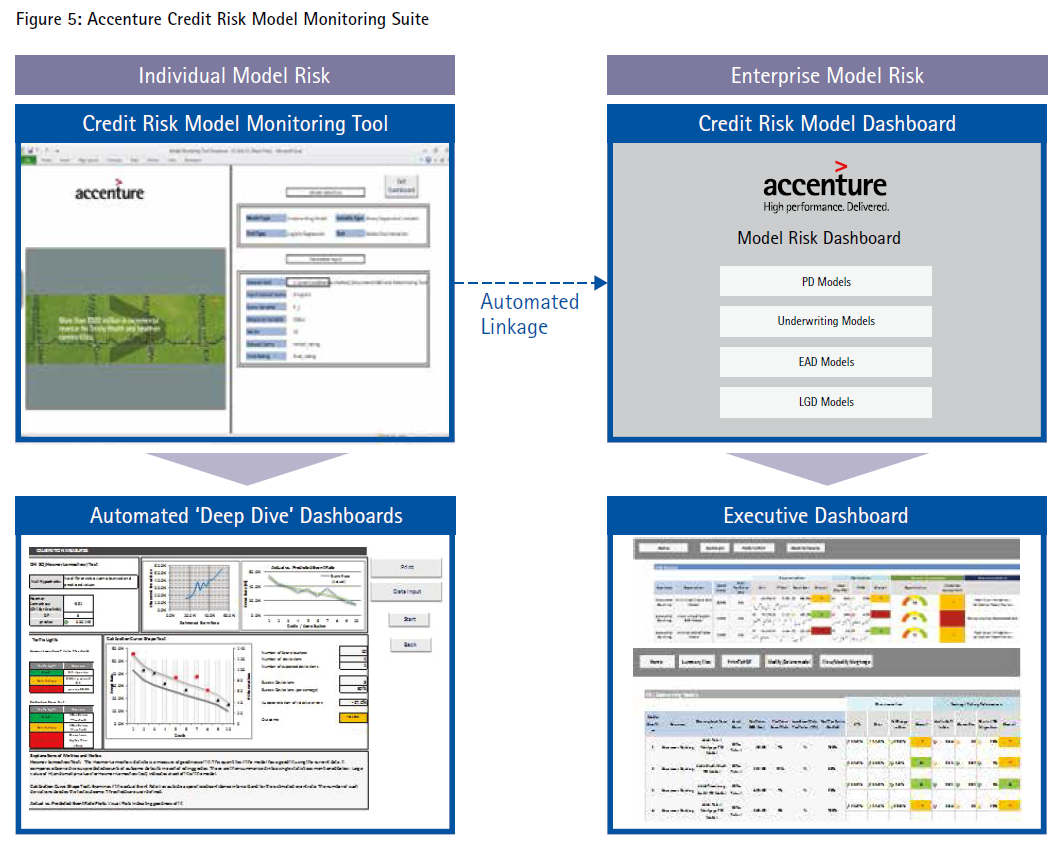
\includegraphics[scale=.3]{images/gov2}
%\end{figure}
%\end{frame}


%\begin{frame}
%\frametitle{Role of validation}
%\begin{itemize}
%	\item 
%\end{itemize}
%\end{frame}
%
%
%\begin{frame}
%\frametitle{The validation process}
%\begin{itemize}
%	\item 
%\end{itemize}
%\end{frame}
%
%
%\begin{frame}
%\frametitle{Model governance and validation}
%\begin{itemize}
%	\item 
%\end{itemize}
%\end{frame}
%
%
%\begin{frame}
%\frametitle{Model change - when and how to validate}
%\begin{itemize}
%	\item 
%\end{itemize}
%\end{frame}
%
%
%\begin{frame}
%\frametitle{Board engagement/communication}
%\begin{itemize}
%	\item 
%\end{itemize}
%\end{frame}


%\begin{frame}
%\frametitle{Change control}
%Models can be subject to minor or major changes at any stage during their life cycle.
%\begin{figure}[h]
%	\centering
%	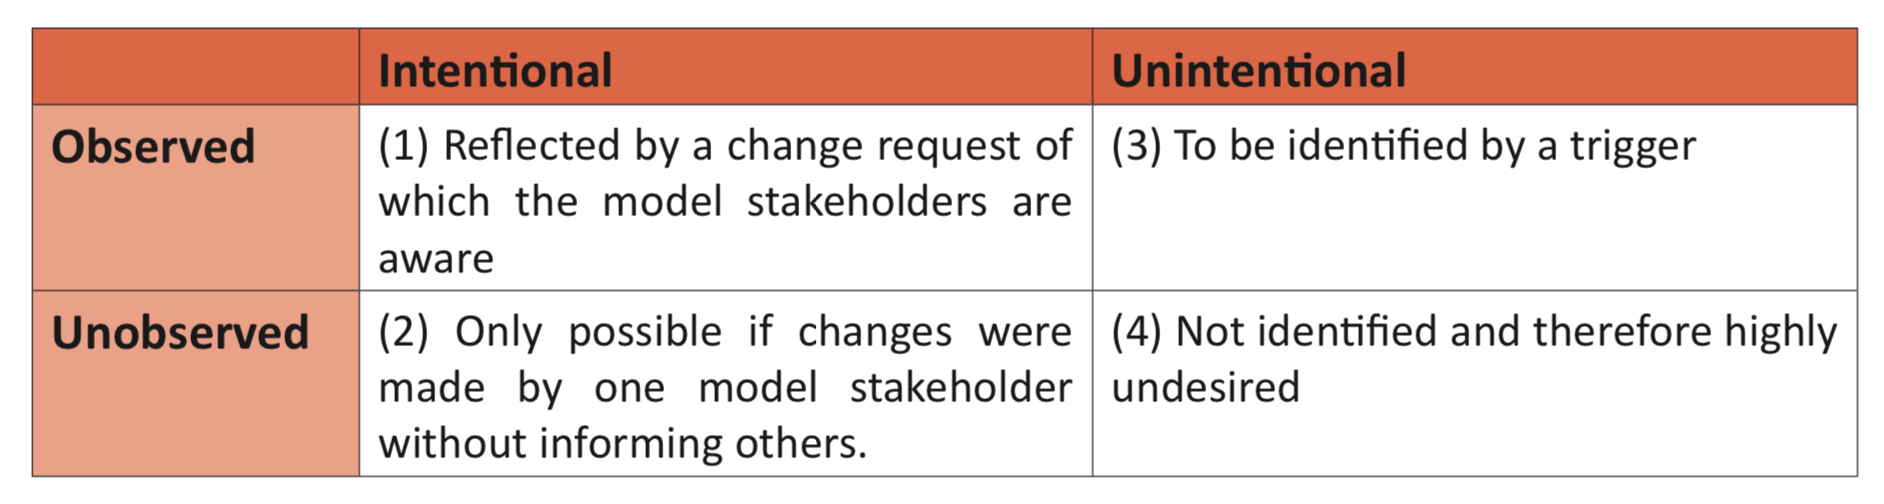
\includegraphics[scale=.3]{images/change_control}
%\end{figure}
%Unobserved and unintentional changes (4) represent serious model risk. Therefore, this type of changes must be minimized at all times.
%All changes can be classified in terms of impact into for example: Small, Medium, Large and Urgent.
%\end{frame}


%\begin{comment}
%- explain methodology, key assumptions and parameters
%- document the nature of the data used, and material assumptions and parameters used in the model
%- design, theory, and logic underlying the model
%- intended purpose of the models and how the user’s needs are addressed by those models
%- clear statement of purpose to ensure that the model development is aligned with its intended purpose
%- statement about any purposes for which the model is not appropriate
%- the extent to which a model fails to fulfill its intended purpose, due to limited information, time constraints, or other practical consideration; 
%- any other known material limitations of the models that have been used and the implications of those limitations.
%- documenting the calculations and programming code over which they have control or responsibility.
%- The extent of documentation would differ depending on whether they are using purchased software or a homegrown system.
%- In the case of purchased software (externally developed), consider requesting documentation of the calculations or code to support reliance on the purchased software.
%- use appropriate governance and controls to minimize model risk, to maintain the integrity of the model, and to avoid the introduction or use of unintentional or untested changes
%- Document: 
%	o Roles \& Responsibilities—Define and document responsibilities for various roles in the governance of the model;
%	o Document Access Controls — Processes for limiting access through access authorization and periodic access review;
%	o State Change Control Procedures—Processes for authorizing changes to the model, reviewing and testing those changes, and where appropriate implementing system controls to segregate the testing and production environments;
%	o Document Model Review Process—Process for reviewing and documenting various validation activities; and
%	o Model Review Sign-off—Maintain sign-off documentation for model review.
% A model steward could help to ensure modeling best practices related to documentation, validation, and governance. The role of model steward can provide a segregation of duties between the activities connected with the initial model and the subsequent activities associated with model and system updates, change control management testing, and validation of these models.
% The responsibilities of a model steward could include approval of new models and model changes for promotion to the production environment. Maintenance of testing, quality assurance, and production environments are also potential responsibilities of a model steward.
% Model validation is part of model risk management and quality control and is the practice of performing an independent challenge and thorough assessment of the reasonableness and adequacy of a model based on peer review and testing across multiple dimensions including design, data, assumptions, results, and governance. The assessment provides internal and external users of model results with a level of assurance that the model is fit for purpose and is performing as expected across a range of scenarios with limitations properly documented, is consistent with other internal and external models, and is in line with design objectives, regulations, enterprise standards, ASOPs, and industry practice.
% Some of the testing procedures used by model validation teams to independently assess models may also be used elsewhere in the company to check and gain comfort with models; e.g., model development teams may use the procedures as they build out models, and model production teams may use the same procedures as they put models to use.
%\end{comment}

\begin{frame}
\frametitle{References}
\begin{enumerate}
	\item Model governance [Gustavo Ordonez-­Sanz] (Moody's Analytics, 2014)
	\item 8 Key elements for a solid Model Governance framework [Tony Cartia] (SAS Hidden Insights, 2017)
	\item Credit risk model monitoring [Larry Lerner; Parvez Shaikh; Tadhg O’Suilleabhain; Siddhartha Chatterji] (Accenture, 2014)
	\item Emerging trends in model risk management [Luther Klein; Michael Jacobs Jr; Akber Merchant] (Accenture, 2015)
	\item Model governance [Hans Heintz] (Riskquest, 2012)
	\item Model governance - some consideration for practising life actuaries [Model Governance Practice Note Work Group of the American Academy of Actuaries] (2017)
	\item Internal model validation - governance and operating model [Institute of Risk Management] (2014)
	\item Model governance [Robert L. Burns] (Supervisory Insights, 2005)
\end{enumerate}
\end{frame}

\end{document}